\documentclass[12pt,a4paper,oneside]{report}

% ---------- idioma e fontes
\usepackage[T1]{fontenc}
\usepackage[utf8]{inputenc}
\IfFileExists{portuges.ldf}{\usepackage[brazilian]{babel}}{\usepackage[provide=*,brazilian]{babel}}
\IfFileExists{newtxtext.sty}{\usepackage{newtxtext}\usepackage{newtxmath}}{\usepackage{mathptmx}\usepackage{amssymb}}
\usepackage{amsmath,mathtools}

% ---------- pagina (ABNT: 3 cm sup./esq., 2 cm inf./dir.)
\usepackage[top=3cm,left=3cm,bottom=2cm,right=2cm,headheight=15pt,headsep=0.75cm]{geometry}
\usepackage{setspace}
\onehalfspacing
\usepackage{indentfirst}
\setlength{\parindent}{1.25cm}
\setlength{\parskip}{0pt}

% ---------- paragrafos nunca divididos entre paginas
\interlinepenalty=10000
\clubpenalty=10000
\widowpenalty=10000
\postdisplaypenalty=10000
\displaywidowpenalty=10000
\predisplaypenalty=10000
\raggedbottom

% ---------- tabelas, figuras, legendas
\usepackage{graphicx,longtable}
\usepackage{tikz}
\usetikzlibrary{positioning,arrows.meta,patterns}
\usepackage{pgfplots}
\pgfplotsset{compat=1.16}
\usepackage{booktabs,tabularx,array}
\usepackage[section]{placeins}
\usepackage{caption}
\usepackage{subcaption}
\usepackage{float}
\captionsetup{font={small},labelsep=endash,justification=centering,skip=6pt}
\captionsetup[table]{position=top}
\counterwithout{figure}{chapter}
\counterwithout{table}{chapter}
\counterwithout{equation}{chapter}
\renewcommand{\figurename}{Figura}
\renewcommand{\tablename}{Tabela}
\newcommand{\fonte}[1]{\par\vspace{4pt}{\footnotesize\centering Fonte: #1\par}}
\newcommand{\nota}[1]{\par\vspace{2pt}\noindent\begin{minipage}{\linewidth}\footnotesize\setlength{\parindent}{0pt}Nota: #1\end{minipage}\par}
\setlength{\textfloatsep}{14pt plus 2pt minus 2pt}
\setlength{\floatsep}{14pt plus 2pt minus 2pt}

% ---------- titulos (ABNT: numeracao progressiva, alinhados a esquerda)
\usepackage{titlesec}
\setcounter{secnumdepth}{3}
\setcounter{tocdepth}{3}
\titleformat{\chapter}{\normalfont\bfseries\MakeUppercase}{\thechapter}{0.5em}{}
\titleformat{name=\chapter,numberless}{\normalfont\bfseries\filcenter}{}{0pt}{}
\titlespacing*{\chapter}{0pt}{0pt}{1.5\baselineskip}
\titleformat{\section}{\normalfont\bfseries}{\thesection}{0.5em}{}
\titlespacing*{\section}{0pt}{1.5\baselineskip}{\baselineskip}
\titleformat{\subsection}{\normalfont\bfseries}{\thesubsection}{0.5em}{}
\titlespacing*{\subsection}{0pt}{1.5\baselineskip}{\baselineskip}
\titleformat{\subsubsection}{\normalfont\bfseries\itshape}{\thesubsubsection}{0.5em}{}
\titlespacing*{\subsubsection}{0pt}{1.5\baselineskip}{\baselineskip}
\newcommand{\pretextualchapter}[1]{\clearpage\chapter*{#1}}

% ---------- sumario e listas
\usepackage{tocloft}
\AtBeginDocument{%
  \renewcommand{\contentsname}{SUMÁRIO}%
  \renewcommand{\listfigurename}{LISTA DE FIGURAS}%
  \renewcommand{\listtablename}{LISTA DE TABELAS}%
  \renewcommand{\figurename}{Figura}%
  \renewcommand{\tablename}{Tabela}%
  \renewcommand{\bibname}{REFERÊNCIAS}}
\renewcommand{\cfttoctitlefont}{\hfill\normalfont\bfseries}
\renewcommand{\cftaftertoctitle}{\hfill}
\renewcommand{\cftloftitlefont}{\hfill\normalfont\bfseries}
\renewcommand{\cftafterloftitle}{\hfill}
\renewcommand{\cftlottitlefont}{\hfill\normalfont\bfseries}
\renewcommand{\cftafterlottitle}{\hfill}
\setlength{\cftbeforetoctitleskip}{0pt}
\setlength{\cftbeforeloftitleskip}{0pt}
\setlength{\cftbeforelottitleskip}{0pt}
\renewcommand{\cftchapleader}{\cftdotfill{\cftdotsep}}
\renewcommand{\cftchapfont}{\bfseries}
\renewcommand{\cftchappagefont}{\bfseries}
\setlength{\cftbeforechapskip}{4pt}
\setlength{\cftsecindent}{0pt}\setlength{\cftsubsecindent}{0pt}\setlength{\cftsubsubsecindent}{0pt}
\setlength{\cftchapnumwidth}{1.5em}\setlength{\cftsecnumwidth}{2.5em}
\setlength{\cftsubsecnumwidth}{3.2em}\setlength{\cftsubsubsecnumwidth}{4em}
\renewcommand{\cftfigpresnum}{Figura~}
\renewcommand{\cftfigaftersnum}{~--}
\setlength{\cftfigindent}{0pt}\setlength{\cftfignumwidth}{5.5em}
\renewcommand{\cfttabpresnum}{Tabela~}
\renewcommand{\cfttabaftersnum}{~--}
\setlength{\cfttabindent}{0pt}\setlength{\cfttabnumwidth}{5.5em}

% ---------- rodape: numero da pagina centralizado embaixo
\usepackage{fancyhdr}
\fancypagestyle{textual}{\fancyhf{}\fancyfoot[C]{\small\thepage}\renewcommand{\headrulewidth}{0pt}}
\fancypagestyle{plain}{\fancyhf{}\renewcommand{\headrulewidth}{0pt}}

\usepackage[authoryear,round]{natbib}
\usepackage{xurl}
\newcommand{\linkcnes}[1]{\href{#1}{\texttt{cnes2.datasus.gov.br} (competência 07/2026)}}
\usepackage{enumitem,needspace}
\usepackage[hidelinks]{hyperref}
\hypersetup{pdftitle={Planejamento da rede de atenção à saúde de Itaúna},
  pdfauthor={Thais Pereira de Oliveira, Pedro Martins de Souza, Luana Soares Ottoni}}

\setlength{\emergencystretch}{2em}
\renewcommand{\bibname}{Referências}

% =====================================================================
% Identificacao do trabalho
\newcommand{\instituicao}{Universidade Federal de Minas Gerais}
\newcommand{\curso}{Escola de Engenharia -- Departamento de Engenharia de Produção}
\newcommand{\autores}{Thais Pereira de Oliveira\\Pedro Martins de Souza\\Luana Soares Ottoni}
\newcommand{\orientador}{Prof. João Flávio de Freitas Almeida}
\newcommand{\cidade}{Belo Horizonte}
\newcommand{\ano}{2026}
\newcommand{\titulo}{Planejamento da rede de atenção à saúde de Itaúna}
\newcommand{\subtitulo}{localização de UBS e alocação hierárquica de encaminhamentos em uma abordagem sequencial}
% =====================================================================

\begin{document}
\hypersetup{pageanchor=false}

% ---------- capa
\begin{titlepage}
\centering
{\bfseries\MakeUppercase{\instituicao}\par}
{\MakeUppercase{\curso}\par}
\vspace{2.5cm}
{\bfseries\MakeUppercase{\autores}\par}
\vfill
{\bfseries\large\MakeUppercase{\titulo}:\par}
{\large\subtitulo\par}
\vfill
{\MakeUppercase{\cidade}\par}
{\ano\par}
\end{titlepage}

% ---------- folha de rosto
\begin{titlepage}
\centering
{\bfseries\MakeUppercase{\autores}\par}
\vspace{4cm}
{\bfseries\large\MakeUppercase{\titulo}:\par}
{\large\subtitulo\par}
\vspace{2cm}
\hspace*{.45\linewidth}\begin{minipage}{.55\linewidth}
\singlespacing\small
Trabalho apresentado à disciplina EPD919 -- Pesquisa Operacional para Saúde, do Departamento de
Engenharia de Produção da Escola de Engenharia da \instituicao{}, no período 2026/2, como requisito
parcial para aprovação.\par
\vspace{8pt}
\orientador.
\end{minipage}
\vfill
{\MakeUppercase{\cidade}\par}
{\ano\par}
\end{titlepage}

\hypersetup{pageanchor=true}
\pagestyle{textual}
\fancypagestyle{plain}{\fancyhf{}\fancyfoot[C]{\small\thepage}\renewcommand{\headrulewidth}{0pt}}

\chapter*{Resumo}
Este trabalho aplica modelos de Pesquisa Operacional ao planejamento da rede de saúde de Itaúna (MG) em
duas etapas. Na primeira, um modelo de programação linear inteira mista escolhe onde abrir novas Unidades
Básicas de Saúde (UBS) e quantas equipes de Saúde da Família (eSF) e agentes comunitários de saúde (ACS)
alocar. Os objetivos seguem uma ordem de prioridade, que maximiza primeiro a cobertura até 3 km, depois
minimiza o custo em cinco anos e, por fim, a distância. Equipes móveis atendem os pontos que continuam
fora desse raio. Na segunda etapa, a demanda especializada, estimada pela produção ambulatorial e
hospitalar dos moradores em 2025, é encaminhada das UBS aos estabelecimentos secundários e terciários
existentes. A base tem 91 pontos territoriais, 22 UBS e 104.002 habitantes projetados para 2026. O plano
abre nove UBS e chega a 39 eSF e 192 ACS, o que eleva a cobertura com capacidade de 65,6\% para 97,7\%, e
duas equipes móveis levam a cobertura potencial a 100\%. O funcionamento custa R\$ 3,00 milhões por mês, o que equivale a 70,7\% da dotação anual da Atenção
Básica, e a construção exige um investimento único de R\$ 22,8 milhões. Na rede especializada, a média
complexidade ambulatorial é quase toda atendida no município, mas cerca de 25\% da alta complexidade não
cabe na oferta local. As UBS rurais ficam com 17\% a 52\% de ocupação, o que mostra o custo
da equidade territorial.

\noindent\textbf{Palavras-chave:} localização de instalações; atenção primária à saúde; máxima cobertura;
rede hierárquica; otimização lexicográfica.

\chapter*{Abstract}
This study applies Operations Research models to plan the health care network of Itaúna, Brazil, in two
sequential stages. First, a mixed-integer linear program with lexicographic objectives locates new
primary care units (UBS) and sizes family health teams and community health workers, maximizing
coverage within 3 km, then minimizing five-year cost and, finally, travel distance. Mobile teams
complement the points still outside the radius. Second, a flow model allocates elective specialized
demand, estimated from 2025 outpatient and inpatient records of residents, to existing secondary and
tertiary providers. The plan selects 9 new units, 39 teams and 192 community health workers, raising
capacity-constrained potential coverage from 65.6\% to 97.7\% (100\% with two mobile teams), at an estimated operating cost of R\$ 3.00 million per month, equal to 70.7\% of the annual primary care budget, plus R\$ 22.8 million in construction. About 25\% of
high-complexity outpatient demand remains unallocated. Allowing two care levels in two providers
reduces this gap to 20\%. Rural units show low occupancy, illustrating the cost of territorial equity.

\noindent\textbf{Keywords:} facility location; primary health care; maximal covering; hierarchical network;
lexicographic optimization.

\FloatBarrier
\clearpage\tableofcontents\clearpage\listoftables\clearpage\listoffigures\clearpage

% =====================================================================
\chapter{Introdução}

A atenção primária é o primeiro contato da população com o sistema de saúde e coordena o cuidado
prestado nos demais níveis \citep{mendes2010}. No Sistema Único de Saúde (SUS), a Unidade Básica de
Saúde (UBS) é a porta de entrada preferencial da rede, e a Política Nacional de Atenção Básica (PNAB)
estabelece referências de população por equipe e por agente comunitário de saúde \citep{pnab2017}. A
Estratégia Saúde da Família é a forma prioritária de expansão e consolidação da atenção primária no SUS
\citep{pnab2017}.

A atenção secundária reúne serviços especializados de complexidade intermediária, enquanto a
terciária concentra recursos de maior complexidade \citep{mendes2010}. Uma internação não é necessariamente terciária, pois pode envolver procedimentos
de média ou de alta complexidade. Por exigirem
profissionais e equipamentos escassos, esses serviços são concentrados em polos regionais, segundo o
princípio de economia de escala das Redes de Atenção à Saúde \citep{brasil2010}. O acesso a eles ocorre
por referenciamento, em que a UBS encaminha parte dos usuários ao nível secundário e parte destes segue
ao terciário \citep{brasil2011,sahin2007}. Por isso, ao expandir a atenção primária, é preciso verificar se os serviços
especializados comportam a demanda encaminhada.

A utilização corresponde aos atendimentos realizados, enquanto o acesso envolve as condições para
receber o cuidado, como localização, capacidade e organização dos serviços
\citep{aday1974,santana2023}. Os registros de produção mostram o uso da rede e servem para dimensionar a
oferta que mantém esse padrão de atendimento na população projetada. Eles não captam, porém, a
necessidade que não chegou aos serviços \citep{santana2023}.

Planejar essa rede exige decidir onde instalar unidades, quanta capacidade alocar e como encaminhar
a população entre os níveis. A Pesquisa Operacional oferece modelos de localização e alocação para
apoiar essas decisões em saúde
\citep{daskin2004,ahmadi2017}, inclusive em redes com vários níveis de serviço \citep{sahin2007,hodgson1988}. Em
Itaúna, a base territorial combina bairros e setores censitários urbanos e rurais, com
populações de tamanhos muito diferentes, e alguns estabelecimentos oferecem serviços de mais de um nível de atenção. Essas
características motivam regras de abertura distintas para UBS urbanas e rurais e a comparação de formas
de classificar a rede especializada.

O objetivo deste trabalho é propor um plano de expansão da atenção primária de Itaúna e avaliar como a
demanda especializada gerada pela rede proposta pode ser distribuída entre os estabelecimentos
secundários e terciários existentes. São definidas novas UBS, equipes de Saúde da Família (eSF) e agentes
comunitários de saúde (ACS), com avaliação de cobertura, custos, distâncias e impacto orçamentário.
Busca-se, além disso, quantificar o custo de ampliar a cobertura nas áreas rurais e identificar a parcela
da demanda especializada que a oferta local não comporta.

O estudo adota uma abordagem sequencial. Na primeira etapa, são definidas a localização das novas UBS,
as equipes e os ACS, além de equipes móveis para os pontos que ficam a mais de 3 km de uma UBS. Na segunda, o
plano de atenção primária fixa a origem dos encaminhamentos, que são distribuídos entre os
estabelecimentos especializados. Procedimentos ambulatoriais e internações são analisados separadamente.
O Capítulo~2 revisa a literatura, o Capítulo~3 descreve dados e modelos, o Capítulo~4 apresenta e
discute os resultados, e o Capítulo~5 reúne as conclusões.

% =====================================================================
\chapter{Revisão bibliográfica}

\Needspace{12\baselineskip}
\section{O SUS e as redes de atenção à saúde}

O Sistema Único de Saúde (SUS) foi criado com base nos princípios de universalidade, integralidade e
equidade, e é organizado de forma descentralizada, regionalizada e hierarquizada em níveis de
complexidade crescente \citep{brasil1990,paim2011}. \citet{castro2019} mostram que, em seus primeiros
30 anos, o SUS ampliou o acesso universal sobretudo por meio da atenção primária, mas ainda enfrenta
desigualdades geográficas persistentes e financiamento insuficiente, desafios que motivam este trabalho.
Para apoiar o planejamento, a Portaria nº 1.631/2015 estabelece parâmetros para a programação de ações
e serviços no SUS e admite sua adequação às realidades locais \citep{brasil2015a}.

\citet{mendes2010} propõe as Redes de Atenção à Saúde (RAS) como resposta à fragmentação dos sistemas.
As RAS são compostas por uma população adscrita, uma estrutura operacional de pontos de atenção e um
modelo de atenção, e têm a atenção primária como centro de comunicação que coordena os fluxos entre os
níveis secundário e terciário. A Portaria nº 4.279/2010 estabelece as diretrizes das RAS e adota como
fundamentos a economia de escala, a disponibilidade de recursos e a integração entre os níveis. Por esses
fundamentos, recursos escassos devem ser concentrados e os menos escassos, distribuídos \citep{brasil2010}.

O Decreto nº 7.508/2011 define a atenção primária como porta de entrada e ordenadora do acesso aos
serviços especializados, organizados por referenciamento do usuário dentro de regiões de saúde
\citep{brasil2011}. Segundo a PNAB, a eSF é formada por
médico, enfermeiro, auxiliar ou técnico de enfermagem e ACS. A política recomenda de 2.000 a 3.500 pessoas
por equipe e até quatro equipes por UBS, com adequações ao território, e até 750 pessoas por ACS em áreas
de grande dispersão, risco ou vulnerabilidade \citep{pnab2017}. \citet{freire2021} analisam como a PNAB
de 2017 afetou o número de ACS na atenção primária brasileira.

\Needspace{12\baselineskip}
\section{Acesso, necessidade e acessibilidade}

Reduzir custos não basta quando a população não consegue receber o atendimento de que precisa, e
por isso o planejamento em saúde também precisa medir o acesso \citep{ahmadi2017}. \citet{aday1974} propõem um quadro em
que o acesso é medido pelo uso dos serviços em relação à necessidade. O modelo relaciona a política de
saúde, as características do sistema, como recursos e organização, e as da população em risco, cujos
resultados são a utilização e a satisfação dos usuários.

\citet{santana2023} distinguem necessidade, demanda e oferta e combinam esses três elementos em sete
situações. Entre elas, há a necessidade e a demanda sem oferta suficiente, em que o atendimento é
restringido pela capacidade, e a oferta sem necessidade nem demanda, que representa capacidade ociosa.
\citet{shengelia2005} definem cobertura efetiva como a probabilidade de um indivíduo obter ganho de saúde
de uma intervenção quando dela necessita, o que integra necessidade, utilização e qualidade.

\citet{guagliardo2004} separa o acesso potencial do realizado e identifica duas dimensões espaciais. A
disponibilidade é o número de pontos de atendimento que o usuário pode escolher, e a acessibilidade é a
dificuldade de deslocamento até eles, medida pela distância ou pelo tempo de viagem. As medidas incluem razões de oferta por
habitante, distância ao serviço mais próximo, distância média e modelos gravitacionais. O modelo
gravitacional mais simples foi proposto por \citet{hansen1959}, e \citet{joseph1982} o ajustaram pela
população concorrente de cada serviço, considerando oferta e demanda simultaneamente.

\Needspace{12\baselineskip}
\section{Localização de instalações de saúde}\label{sec:revlocal}

A localização de instalações é uma das decisões estratégicas mais importantes em saúde, pois unidades
mal localizadas ou em número inadequado aumentam custos e dificultam o acesso \citep{ahmadi2017}. Os
critérios de avaliação de instalações não emergenciais são a eficiência, a efetividade e a equidade, e a
minimização de custos é outro objetivo frequente \citep{ahmadi2017}. Esses problemas envolvem interesses
diferentes. Os pacientes valorizam o deslocamento e o tempo de espera, os prestadores valorizam os custos
e a disponibilidade de pessoal, e a comunidade valoriza a equidade do acesso \citep{contreras2019}.

Os problemas discretos de localização dividem-se em problemas de cobertura, como cobertura de conjuntos,
máxima cobertura e $p$-centro, e problemas de mediana, como $p$-mediana e custo fixo
\citep{daskin2008,daskin2004}. O problema de máxima cobertura, proposto por \citet{church1974}, maximiza
a demanda atendida dentro de uma distância de serviço com um número fixo de instalações. O problema das
$p$-medianas, formulado por \citet{hakimi1964}, minimiza a distância ponderada pela demanda, e o problema
de custo fixo com capacidade acrescenta custos de abertura e limites de atendimento por unidade
\citep{ahmadi2017}.

\citet{contreras2019} descrevem a capacidade das unidades de saúde a partir dos recursos necessários,
como profissionais, leitos e equipamentos. Quando a capacidade é limitada, a demanda de uma região pode
ser repartida entre várias unidades, mas essa alocação múltipla não considera a preferência do paciente.
Restrições de alocação à unidade mais próxima representam essa preferência, ao custo de tornar o
problema mais restrito. \citet{rahman2000} mostram que modelos de localização-alocação apoiam o
planejamento da atenção básica em países em desenvolvimento, em que a acessibilidade geográfica é uma
barreira relevante.

Como os problemas de localização em saúde são multiobjetivo, é preciso decidir como combinar critérios.
Na otimização lexicográfica, os objetivos são ordenados por prioridade. Otimiza-se o primeiro e, com o
seu valor ótimo mantido como restrição, otimizam-se os demais em sequência \citep{ehrgott2005}.
Diferentemente da soma ponderada, essa abordagem não exige pesos entre grandezas de natureza diferente,
como população coberta e custo, mas pressupõe uma ordem de prioridade bem definida.

\Needspace{12\baselineskip}
\section{Redes hierárquicas de serviços de saúde}

\citet{sahin2007} e \citet{contreras2019} classificam os problemas de localização hierárquica por três
características. O padrão de fluxo pode ser de fluxo único, em que o paciente percorre todos os níveis,
ou de fluxo múltiplo, em que pode pular níveis. A hierarquia de serviços pode ser aninhada, quando uma
unidade de nível superior oferece também os serviços dos níveis inferiores, ou não aninhada. A
configuração espacial é coerente quando toda a demanda de uma unidade é encaminhada a uma única unidade
do nível seguinte.

\citet{narula1986} revisa os problemas hierárquicos de mediana aplicados ao planejamento da saúde, entre
eles a formulação de Narula e Ogbu, em que uma proporção dos pacientes atendidos no primeiro nível é
encaminhada ao nível superior. \citet{schultz1970} mostra que o raio de serviço ótimo de cada nível
resulta do equilíbrio entre o benefício por habitante e o custo de produção e deslocamento, e que os
serviços de nível mais alto toleram deslocamentos maiores.

\citet{hodgson1988} argumenta que os níveis de uma rede de atenção estão interligados, de modo que
localizá-los de forma independente pode levar a soluções ruins. O autor também observa que os pacientes
nem sempre procuram a unidade mais próxima, pois a atratividade cresce com o nível do serviço e diminui
com a distância. Essas observações justificam tratar a rede de forma hierárquica e interpretar com
cautela as hipóteses de alocação.

\Needspace{12\baselineskip}
\section{Aplicações à reorganização de redes de saúde}

\citet{guerriero2016} comparam a rede hospitalar existente na Calábria, Itália, com soluções de modelos
clássicos de localização. A rede atual deixava parte da demanda descoberta, enquanto cenários que
realocam a demanda entre hospitais com capacidade expansível permitiam atendê-la integralmente.
\citet{mic2019} localizam centros de atenção primária na Síria com um modelo multiobjetivo que maximiza
a população atendida e minimiza os custos.

\citet{elorza2022} propõem uma metodologia de máxima cobertura baseada na quantificação de necessidade,
oferta e demanda para avaliar e redesenhar redes de atenção primária. No caso estudado, as unidades
estavam bem distribuídas geograficamente, mas a oferta de serviços não correspondia às necessidades da
população, caracterizando um problema de capacidade, e não de localização. Essa distinção entre
proximidade e capacidade é central para os resultados deste trabalho.

% =====================================================================
\chapter{Metodologia}

\section{Visão geral da abordagem}
A Figura~\ref{fig:fluxo} resume a abordagem, que tem duas etapas resolvidas em sequência. Na primeira,
os dados de população e de produção alimentam o modelo da atenção primária à saúde (APS), que define as
UBS, as equipes e os ACS, e equipes móveis atendem os pontos que continuam distantes de uma UBS. Na
segunda, a demanda especializada é vinculada às UBS, que passam a ser a origem dos encaminhamentos aos
níveis secundário e terciário. Essa sequência permite analisar primeiro a expansão territorial e,
em seguida, a distribuição dos atendimentos especializados na rede definida.

\begin{figure}[htbp]\centering
\begin{tikzpicture}[
  etapa/.style={draw=black!70, line width=0.8pt, rounded corners=4pt, fill=black!4,
    text width=9cm, minimum height=1.4cm, align=center, inner sep=6pt, font=\normalsize},
  seta/.style={-{Stealth[length=7pt,width=6pt]}, line width=0.9pt, black!70,
    shorten >=3pt, shorten <=3pt},
  node distance=0.9cm]
\node[etapa] (dados) {Dados de população e demanda municipal};
\node[etapa, below=of dados] (aps) {Localização das UBS e dimensionamento\\ das equipes da atenção primária};
\node[etapa, below=of aps] (vinc) {População e demanda vinculadas às UBS};
\node[etapa, below=of vinc] (enc) {Encaminhamentos secundários e terciários};
\draw[seta] (dados.south) -- (aps.north);
\draw[seta] (aps.south) -- (vinc.north);
\draw[seta] (vinc.south) -- (enc.north);
\end{tikzpicture}
\caption{Etapas da abordagem sequencial}\label{fig:fluxo}
\fonte{Elaboração própria.}
\end{figure}

\section{Dados e projeção da população}
A base territorial tem 91 pontos, sendo 51 bairros e 40 setores censitários, que somavam 97.669
habitantes no Censo de 2022 \citep{ibge2022}. Os pontos cobrem as áreas urbanas
e rurais, e cada um concentra a população do seu território em uma única coordenada, a partir da qual se
medem as distâncias até as UBS. Essa agregação mantém o modelo pequeno e fácil de interpretar. Como o IBGE não publica estimativas por bairro ou setor, a
participação de cada ponto no total é mantida para projetar 104.002 habitantes em 2026,
conforme a estimativa oficial do IBGE, que era de 103.272 habitantes em 2025 \citep{ibge2025est,ibge2026est}.
As equipes, os profissionais, as salas e os leitos das unidades vêm do Cadastro Nacional de
Estabelecimentos de Saúde (CNES) de julho de 2026 \citep{cnes2026}.

A demanda especializada é estimada pela produção registrada no Sistema de Informações Ambulatoriais (SIA)
e no Sistema de Informações Hospitalares (SIH) em 2025, obtida no DATASUS, o departamento de informática
do SUS \citep{datasus2026,tabnet}. Consideram-se apenas os atendimentos eletivos, isto é, programados, de
moradores de Itaúna, pois são esses que chegam à atenção especializada por encaminhamento da UBS, enquanto
as urgências têm porta de entrada própria. Na parte ambulatorial, entram 753 procedimentos de média e alta complexidade com
finalidade diagnóstica, clínica ou cirúrgica \citep{sigtap}.

As urgências ficam fora da demanda, mas
entram na carga que ocupa os leitos hospitalares. Os volumes são contados em procedimentos e internações, e
não em pacientes, pois uma pessoa pode gerar vários registros. A taxa de utilização usa a população de 2025, o mesmo ano da produção, e é aplicada à
população de 2026, sem ajuste por idade ou risco. A Seção~\ref{sec:ligacao} detalha esse cálculo.

\section{Oferta especializada e capacidades}
Os níveis secundário e terciário são representados pela média e pela alta complexidade dos
procedimentos. O modelo distribui volumes por nível, sem verificar a compatibilidade entre
especialidades. Na análise principal, chamada de classificação única, cada estabelecimento oferece um só
nível. Na análise complementar, chamada de classificação de dois níveis, o Hospital Manoel Gonçalves e o
Centro de Especialidades Médicas e Odontológicas Dr. Ovídio Nogueira Machado oferecem os dois níveis.
Como o centro realizou apenas 920 procedimentos eletivos de alta complexidade em 2025, contra 84.681 de
média, essa oferta recebe um limite próprio.

\subsection{Capacidade ambulatorial}
A capacidade ambulatorial anual de cada estabelecimento é estimada a partir da sua produção. Toma-se a
produção eletiva do mês de maior volume, multiplica-se por 12 e desconta-se a produção anual destinada a
moradores de outros municípios. O mês de maior produção mostra o volume que o estabelecimento já
conseguiu realizar com a estrutura atual, e o desconto reserva a parte da oferta que atende outros
municípios. Na classificação de dois níveis, cada complexidade tem também um limite
próprio, igual ao maior valor entre a sua produção no mês de pico multiplicada por 12 e a sua produção
anual, também sem os não residentes. A soma das duas complexidades respeita o limite total do
estabelecimento.

\subsection{Leitos gerais e UTI}\label{sec:leitos}
O hospital tem 79 leitos SUS de internação geral e 19 de unidade de terapia intensiva (UTI), o que
equivale a 28.835 e 6.935 dias-leito por ano. Os outros atendimentos, inclusive as urgências, ocupam
cerca de 29.634 dias-leito, mas os registros não mostram quanto disso cabe a cada tipo de leito. Por
isso, a disponibilidade de leitos gerais para internações eletivas fica entre zero e 6.136 dias-leito.
O cenário principal adota o extremo conservador, que é zero, e a Seção~\ref{sec:encaminhamentos} testa
também o extremo favorável. As permanências médias, calculadas pelo SIH, são de 5,13 dias na média e
3,33 dias na alta complexidade.

\section{Modelo de localização e dimensionamento das UBS}\label{sec:modeloaps}
O modelo escolhe onde abrir novas UBS e quantas eSF e ACS cada unidade terá. As candidatas, isto é, os
locais possíveis para novas UBS, são os pontos territoriais a mais de 1 km de uma UBS existente. Sejam
$I$ os pontos de demanda, $E$ as UBS existentes, $C$ as candidatas e $J=E\cup C$. $P_i$ é a população do
ponto $i$, e $d_{ij}$ é a distância em linha reta entre o ponto e a UBS, calculada pela fórmula de
Haversine. O parâmetro $H_{ij}$ vale um quando $d_{ij}$ não passa do raio de cobertura, de 3 km no cenário principal.

As variáveis são a população alocada $q_{ij}\geq0$, a abertura $y_j\in\{0,1\}$, os números de eSF e de
ACS $n_j,a_j\in\mathbb{Z}_+$ e a escolha $z_{jp}\in\{0,1\}$ do porte $p$ de cada nova UBS. Nas UBS
existentes, $n_j^0$ e $a_j^0$ são as eSF e os ACS atuais. O porte segue
o Novo PAC Saúde, programa federal de investimento que define o custo de construção conforme o número
de equipes \citep{novopac2025}. As restrições do modelo são as seguintes.
\begin{align}
\sum_j q_{ij}&=P_i &&\forall i\in I,\\
\sum_i q_{ij}&\leq3000\,n_j,\qquad \sum_i q_{ij}\leq750\,a_j &&\forall j\in J,\\
y_j&=1,\quad n_j\geq n_j^0,\quad a_j\geq a_j^0 &&\forall j\in E,\\
y_j\leq n_j&\leq\overline n_j\, y_j &&\forall j\in J,\\
\sum_i H_{ij}q_{ij}&\geq m_j\,y_j &&\forall j\in C,\\
\sum_p z_{jp}&=y_j,\qquad n_j=\sum_p p\,z_{jp} &&\forall j\in C.
\end{align}

\penalty0
A primeira restrição aloca toda a população de cada ponto. A segunda limita a carga de cada UBS a 3.000
habitantes por eSF e a 750 por ACS. O valor de 3.000 é a média por equipe recomendada desde a
PNAB de 2011 \citep{brasil2013teto} e fica dentro da faixa de 2.000 a 3.500 da PNAB atual. O limite de 750 por ACS, indicado pela PNAB para áreas vulneráveis, vale aqui para
todo o município \citep{pnab2017}. O menor desses dois limites é chamado aqui de capacidade efetiva. As UBS existentes continuam abertas e mantêm suas equipes, e o
número de salas de cada uma limita as novas equipes ($\overline n_j$). Uma nova UBS precisa ter pelo menos
2.000 habitantes no raio na zona urbana e 500 na rural ($m_j$), valores definidos pelo estudo. Cada nova
unidade pode ter de uma a quatro equipes, teto que segue a PNAB.

O custo operacional mensal $O$ soma o custo fixo $f_j$, de R\$ 12.000 nas UBS existentes e R\$ 15.000
nas novas, o custo atual de médicos, enfermeiros e técnicos $C_j^0$, as novas eSF, a $c_e$ cada uma, e os ACS, a $c_a$ cada um. O custo fixo
cobre as despesas de funcionamento sem pessoal e é uma hipótese do estudo. O
investimento $B$ soma o custo de construção $b_p$ das novas UBS, e $G$ é a população coberta dentro do
raio.
\begin{align}
G&=\sum_{i,j}H_{ij}q_{ij},\\
O&=\sum_{j\in E}f_j+\sum_{j\in C}f_jy_j+
\sum_j\left[C_j^0+c_e(n_j-n_j^0)+c_aa_j\right],\\
B&=\sum_{j\in C,p}b_pz_{jp}.
\end{align}

\penalty0
O pessoal atual é estimado pelas horas semanais registradas no CNES \citep{cnes2026}. As horas de cada
categoria são divididas por 40, a jornada das eSF na PNAB \citep{pnab2017}, o que dá o número de
profissionais equivalentes. Esse número é multiplicado por uma remuneração mensal de referência, de R\$ 14.000 para médicos, R\$ 5.000 para enfermeiros, R\$ 3.325 para
técnicos e R\$ 2.375 para auxiliares de enfermagem. Os dois últimos são os pisos nacionais da enfermagem, e
o valor dos enfermeiros fica pouco acima do piso de R\$ 4.750 \citep{brasil2022piso}. O valor dos médicos é
próximo da bolsa-formação bruta do Programa Mais Médicos, de R\$ 14.121,63 em 2026 \citep{maismedicos2026}.

Cada nova eSF tem um médico, um enfermeiro e um técnico. O ACS recebe R\$ 3.242, valor do piso de dois
salários mínimos de 2026, e não o vencimento pago pelo município \citep{brasil2022,brasil2025sm}. Todas
as remunerações são multiplicadas por $(13+1/3)/12\times1{,}30\approx1{,}444$. O primeiro termo
distribui pelos meses o décimo terceiro e o adicional de um terço de férias
\citep{brasil1962decimo,brasil1988cf}. O fator 1,30 soma 20\% de contribuição patronal, 2\% de risco de
acidentes e 8\% de FGTS, como em uma contratação pelo regime CLT \citep{brasil1991custeio,brasil1990fgts}.
A Tabela~\ref{tab:origem_custos} indica quais valores vêm de normas e quais são hipóteses do estudo.
O modelo é resolvido em três fases, seguindo a otimização lexicográfica descrita na Seção~\ref{sec:revlocal}.
\begin{align}
\text{Fase 1}\quad&\max\;G &&\Rightarrow G^*,\\
\text{Fase 2}\quad&\min\;B+60\,O &&\text{s.a. }G=G^*\ \Rightarrow O^*,B^*,\\
\text{Fase 3}\quad&\min\;0{,}05\sum_{i,j}d_{ij}q_{ij}
&&\text{s.a. }G=G^*,\ O\leq1{,}02\,O^*,\ B\leq B^*.
\end{align}

\penalty0
A primeira fase maximiza a população coberta. A segunda minimiza o custo de cinco anos, que soma a
construção a 60 meses de operação a preços constantes, sem reduzir a cobertura obtida. A terceira
minimiza a distância percorrida, aceitando até 2\% a mais de custo operacional e sem aumentar o
investimento. O valor de R\$ 0,05 por habitante-quilômetro serve apenas para ordenar
as soluções pelo deslocamento e não entra no custo operacional. Na implementação, a igualdade $G=G^*$
admite uma tolerância numérica de $10^{-7}$.

O custo operacional também é limitado pelo orçamento da Atenção Básica de 2026. O limite vale para o
acréscimo de funcionamento em relação à rede atual. Sejam $A$ a dotação anual, $C^0$ o custo anual
estimado da rede atual e $R_m$ uma reserva anual para equipes móveis. A restrição é
\begin{equation}
12\left[\sum_{j\in C}f_jy_j+c_e\sum_j(n_j-n_j^0)+c_a\sum_j(a_j-a_j^0)\right]
\leq A-C^0-R_m.
\end{equation}

\penalty0
A dotação vem do RREO de 2026 \citep{tesouro2026}, e $C^0$ usa os mesmos custos unitários do modelo. A
reserva $R_m$ é o custo das equipes móveis de que a rede atual precisaria. A construção entra no custo de cinco anos da segunda fase, mas não nesse limite anual.

Na classificação de \citet{daskin2008}, o modelo combina a máxima cobertura \citep{church1974} com o
problema de custo fixo com capacidade \citep{ahmadi2017}. A capacidade vem dos recursos humanos de cada
unidade, como na modelagem de \citet{contreras2019}. A população de um ponto pode ser dividida entre
várias UBS, sem a exigência de ir à mais próxima, ponto retomado na Seção~\ref{sec:discussao}.

\section{Cobertura e equipes móveis}\label{sec:movel}
Para comparar a rede atual com a proposta, usam-se duas medidas. A cobertura geográfica é a parcela da
população que mora a até 3 km de uma UBS. A cobertura com capacidade é a maior parcela que pode ser
alocada a UBS dentro desse raio sem ultrapassar a capacidade efetiva de cada uma. As duas medidas são
potenciais e não substituem a cobertura oficial do Ministério da Saúde \citep{aps2026} nem a cobertura
efetiva definida por \citet{shengelia2005}.

As equipes móveis atendem os pontos que continuam a mais de 3 km de uma UBS depois do plano. Cada equipe
parte de uma UBS de apoio, chamada de UBS-base, e acompanha até 2.000 habitantes em até cinco pontos, a no máximo
15 km em linha reta da base. Esses três limites são hipóteses do estudo, pois não há parâmetro oficial para
esse arranjo. O modelo maximiza a população atendida e depois minimiza o número de equipes, com
um ACS para cada 750 habitantes atendidos. Essas equipes são adicionais às fixas, e o seu custo inclui
pessoal e encargos, mas não veículos nem combustível.

Sejam $w_{iu}$ a população do ponto $i$ atendida
pela base $u$, $k_u$ o número de equipes móveis da base e $h_{iu}$ um indicador de que a base visita o
ponto. Só podem ser ligados os pontos sem cobertura geográfica e as UBS do plano a até 15 km deles, e os
demais pares têm $w_{iu}=h_{iu}=0$. As variáveis são $w_{iu}\geq0$, $h_{iu}\in\{0,1\}$ e $k_u$ inteiro, e
as restrições são as seguintes.
\begin{align}
\sum_u w_{iu}&\leq P_i,\\
w_{iu}&\leq P_i\,h_{iu},\\
\sum_i w_{iu}&\leq2000\,k_u,\qquad\sum_i h_{iu}\leq5\,k_u.
\end{align}

\penalty0
O limite de pontos vale para a base como um todo, de modo que duas equipes podem visitar até dez pontos.
O modelo não define a rota nem a divisão das visitas entre as equipes.


\section{Encaminhamento hierárquico}\label{sec:enc}

\subsection{Da produção registrada à demanda de cada UBS}\label{sec:ligacao}
A ligação entre a atenção primária e os níveis especializados é feita em quatro passos. Primeiro, a
produção eletiva dos moradores em 2025 é dividida pela população de 2025, o que gera uma taxa de
utilização por habitante para cada grupo de atendimento (Tabela~\ref{tab:taxas}). Os grupos separam
procedimentos ambulatoriais e internações de média e de alta complexidade. Segundo, a taxa é
multiplicada pela população projetada de cada ponto, o que dá a demanda do ponto em 2026,
\begin{equation}
D^n_{ik}=\frac{R^n_k}{P^{2025}}\,P_i,\label{eq:demanda}
\end{equation}
em que $n\in\{2,3\}$ é o nível, $k\in\{\mathrm{AMB},\mathrm{HOSP}\}$ é o tipo de atendimento, $R^n_k$ é a
produção registrada em 2025 e $P^{2025}$ é a população municipal de 2025.

\begin{table}[H]\centering
\caption{Taxas de utilização e demanda especializada projetada}\label{tab:taxas}
\begin{tabular}{lrrr}\toprule
Grupo & Registrado (2025) & Taxa por mil hab. & Demanda (2026)\\\midrule
Ambulatorial, média & 190.856 & 1.848,1 & 192.205,1\\
Ambulatorial, alta & 15.752 & 152,5 & 15.863,3\\
Internação, média & 1.065 & 10,3 & 1.072,5\\
Internação, alta & 350 & 3,4 & 352,5\\
\bottomrule\end{tabular}
\fonte{SIA e SIH \citep{datasus2026}, com população de \citet{ibge2025est} e \citet{ibge2026est}.}
\nota{Taxa = registrado em 2025 / 103.272 habitantes. Demanda em 2026 = taxa $\times$ 104.002 habitantes,
distribuída entre os 91 pontos proporcionalmente à população.}
\end{table}

Terceiro, a demanda de cada ponto acompanha a sua população na alocação feita pelo modelo da atenção
primária. Se o modelo vincula uma fração $\alpha_{iu}$ da população do ponto $i$ à UBS $u$, essa UBS
passa a ser a origem da mesma fração da demanda do ponto. Os moradores atendidos pelas equipes móveis
ficam vinculados à UBS-base, sem dupla contagem, de modo que $\sum_u\alpha_{iu}=1$ e toda a demanda tem
uma UBS de origem. Quarto, o modelo de encaminhamento distribui a demanda de cada UBS entre os
estabelecimentos secundários e terciários, respeitando as suas capacidades.

Como exemplo, com as taxas da Tabela~\ref{tab:taxas}, um ponto com 1.000 moradores gera por ano cerca de 1.848 procedimentos ambulatoriais de
média complexidade, 153 de alta, 10,3 internações de média e 3,4 de alta. Se o modelo vincular 60\%
desses moradores à UBS A e 40\% à UBS B, cada uma encaminhará a mesma proporção desses volumes. No
cenário em que metade da alta complexidade passa antes pelo nível secundário, metade dos 153
procedimentos vai primeiro a esse nível e a outra metade segue direto ao terciário. Os valores podem
ser fracionários porque representam atendimentos esperados.

\subsection{Modelo de encaminhamento}
Não há dados sobre o caminho de cada paciente entre os níveis. Por isso, testam-se três cenários para a
parcela $r$ da demanda de alta complexidade que passa antes pelo nível secundário, igual a 25\%, 50\% ou
75\%. Considera-se ainda que essa parcela já está contida na demanda secundária registrada, para não
contar o mesmo atendimento duas vezes. Para cada ponto $i$ e tipo $k$,
a demanda se divide em três fluxos.
\begin{align}
A_{ik}&=D^2_{ik}-rD^3_{ik},&L_{ik}&=(1-r)D^3_{ik},&V_{ik}&=rD^3_{ik}.
\end{align}

\penalty0
O fluxo $A$ termina no nível secundário, $L$ segue direto ao terciário e $V$ passa pelos dois níveis. Na
classificação de \citet{sahin2007}, a rede tem fluxo múltiplo, pois parte da demanda pula o nível
secundário, e não é coerente, pois a demanda de uma UBS pode ir a vários estabelecimentos. A classificação
única corresponde a uma hierarquia não aninhada, e a de dois níveis torna aninhados o hospital e o centro
de especialidades. O uso de uma proporção fixa de encaminhamento segue os modelos
hierárquicos revisados por \citet{narula1986}.

Sejam $S$ e $T$ os estabelecimentos secundários e terciários, com índices $s$ e $t$. Os fluxos $f$, $g$ e
$v$ levam as parcelas $A$, $L$ e $V$ de cada ponto $i$, vinculado à UBS $u$, até esses estabelecimentos, e as variáveis $\ell$ medem a parte que
fica sem atendimento, chamada de falta. Todas essas variáveis são não negativas, e as equações de
conservação são as seguintes.
\begin{align}
\sum_s f_{iuks}+\ell^f_{iuk}&=A_{ik}\alpha_{iu},\\
\sum_t g_{iukt}+\ell^g_{iuk}&=L_{ik}\alpha_{iu},\\
\sum_{s,t}v_{iukst}+\ell^v_{iuk}&=V_{ik}\alpha_{iu}.
\end{align}

\penalty0
Cada estabelecimento $a$ recebe as cargas $Q^2_{ak}$ e $Q^3_{ak}$, e a carga de um nível que ele não
oferece é zero.
\begin{align}
Q^2_{ak}&=\sum_{i,u}f_{iuka}+\sum_{i,u,t}v_{iukat},\\
Q^3_{ak}&=\sum_{i,u}g_{iuka}+\sum_{i,u,s}v_{iuksa}.
\end{align}

\penalty0
As cargas respeitam o limite ambulatorial total $C_a$, os limites por complexidade $C_a^2$ e $C_a^3$ e os
dias-leito gerais disponíveis $B_a^{geral}$, com permanências médias $\tau_2$ e $\tau_3$.
Os fluxos hospitalares são permitidos apenas nos estabelecimentos identificados como hospitais.
\begin{align}
Q^2_{a,\mathrm{AMB}}+Q^3_{a,\mathrm{AMB}}&\leq C_a,\\
Q^2_{a,\mathrm{AMB}}&\leq C_a^2,\qquad Q^3_{a,\mathrm{AMB}}\leq C_a^3,\\
\tau_2Q^2_{a,\mathrm{HOSP}}+\tau_3Q^3_{a,\mathrm{HOSP}}&\leq B_a^{geral}.
\end{align}

\penalty0
O modelo primeiro minimiza a falta total. Cada falta é dividida pelo total do seu grupo, $N^n_k$, para que
procedimentos e internações não sejam somados como se fossem equivalentes.
\begin{equation}
\Phi=\sum_{i,u,k}\frac{\ell^f_{iuk}+\ell^v_{iuk}}{N^2_k}
+\sum_{i,u,k}\frac{\ell^g_{iuk}+\ell^v_{iuk}}{N^3_k},\qquad N^n_k=\sum_iD^n_{ik}.
\end{equation}

\penalty0
Depois, mantendo a menor falta encontrada, $\Phi^*$, o modelo minimiza a distância percorrida, também
dividida pelos totais de cada grupo. Cada fluxo percorre a distância do ponto à UBS e da UBS ao
estabelecimento, e o fluxo $V$ percorre ainda a distância $d_{st}$ entre os dois níveis, que é zero quando
eles ficam no mesmo estabelecimento.
\begin{align}
Z={}&\sum_{i,u,k,s}\frac{(d_{iu}+d_{us})f_{iuks}}{N^2_k}
+\sum_{i,u,k,t}\frac{(d_{iu}+d_{ut})g_{iukt}}{N^3_k}\nonumber\\
&+\sum_{i,u,k,s,t}\left(\frac{d_{iu}+d_{us}}{N^2_k}+\frac{d_{st}}{N^3_k}\right)v_{iukst}.
\end{align}

\penalty0
Como a falta é minimizada primeiro, a redução da distância nunca é obtida à custa de atender menos no
total, embora a falta possa mudar de um grupo para outro. O modelo não abre novos estabelecimentos
especializados, e as distâncias, em linha reta, servem para comparar configurações da rede, e não para
estimar o tempo real de viagem.

\section{Hipóteses de planejamento}
A Tabela~\ref{tab:hipoteses} resume os parâmetros adotados. Alguns vêm de normas, como os da PNAB
\citep{pnab2017}, outros de valores de referência de custo, como os do Novo PAC Saúde
\citep{novopac2025}, e os demais são hipóteses do estudo. A análise de sensibilidade varia os raios, o crescimento populacional, o mínimo rural e a folga de custo, e os demais parâmetros ficam fixos. Os
parâmetros da PNAB são aplicados de modo uniforme, sem diferenciar a vulnerabilidade social ou as
condições locais de cada território.

\begin{table}[htbp]\centering
\caption{Parâmetros de planejamento e sua origem}\label{tab:hipoteses}
\begin{tabular}{p{.26\linewidth}p{.19\linewidth}p{.44\linewidth}}
\toprule Parâmetro & Valor principal & Origem e observação\\\midrule
Capacidade por eSF & 3.000 habitantes & Média recomendada desde a PNAB de 2011 e dentro da faixa de 2.000 a 3.500 da PNAB atual \citep{brasil2013teto,pnab2017}\\
Habitantes por ACS & 750 & Máximo da PNAB para áreas de maior dispersão ou vulnerabilidade, aplicado a todo o município\\
Raio de cobertura & 3 km & Hipótese do estudo, pois não há padrão oficial de distância. Os valores de 2 e 5 km são testados\\
Distância & Linha reta & Fórmula de Haversine, que dispensa uma base de vias e de tempos de viagem\\
Distância mínima entre candidata e UBS existente & 1 km & Hipótese do estudo, para que a nova UBS não divida a mesma área de uma existente\\
Mínimo para abrir UBS urbana & 2.000 habitantes & Limite inferior da faixa da PNAB, para que a nova equipe tenha população suficiente\\
Mínimo para abrir UBS rural & 500 habitantes & Hipótese do estudo, para permitir UBS em setores rurais pequenos. Os valores 0 e 1.000 são testados\\
Equipes por nova UBS & De 1 a 4 & Teto da PNAB e portes I a IV do Novo PAC Saúde\\
Folga operacional & 2\% & Hipótese do estudo, que permite reduzir a distância com pouco aumento de custo. O valor de 5\% é testado\\
Horizonte de custo & 5 anos & Hipótese do estudo, para somar construção e operação na mesma base, a preços constantes e sem desconto\\
Parcela da alta complexidade via secundária & 25, 50 e 75\% & Cenários, pois não há dados de encaminhamento por paciente\\
Capacidade da equipe móvel & 2.000 habitantes & Hipótese do estudo, igual ao limite inferior da faixa da PNAB por equipe\\
Alcance da equipe móvel & 15 km e 5 pontos & Hipótese do estudo, sem parâmetro oficial para equipes móveis\\
Peso da distância no índice & $\beta=1$ e $2$ & Sensibilidade, pois exige calibração empírica \citep{guagliardo2004}\\
\bottomrule\end{tabular}
\fonte{Elaboração própria, com base em \citet{pnab2017} e \citet{novopac2025}.}
\end{table}

\begin{table}[htbp]\centering
\caption{Origem dos parâmetros monetários e de pessoal}\label{tab:origem_custos}
\begin{tabular}{p{.26\linewidth}p{.23\linewidth}p{.40\linewidth}}
\toprule Parâmetro & Valor adotado & Origem e cálculo\\\midrule
Médico & R\$ 14.000/mês & Próximo da bolsa-formação bruta do Mais Médicos, de R\$ 14.121,63 em 2026 \citep{maismedicos2026}.\\
Enfermeiro & R\$ 5.000/mês & Hipótese do estudo, pouco acima do piso nacional de R\$ 4.750 \citep{brasil2022piso}.\\
Técnico de enfermagem & R\$ 3.325/mês & Piso nacional, 70\% do piso do enfermeiro, pelo valor integral \citep{brasil2022piso}.\\
Auxiliar de enfermagem & R\$ 2.375/mês & Piso nacional, 50\% do piso do enfermeiro, pelo valor integral \citep{brasil2022piso}.\\
ACS & R\$ 3.242/mês & Piso constitucional de dois salários mínimos de 2026, de R\$ 1.621 cada \citep{brasil2022,brasil2025sm}.\\
Provisões anuais & $(13+1/3)/12$ & Décimo terceiro e um terço de férias distribuídos nos 12 meses \citep{brasil1962decimo,brasil1988cf}.\\
Encargos sobre a base & 30\% & 20\% de contribuição patronal, 2\% de risco e 8\% de FGTS, aplicados a todos os vínculos \citep{brasil1991custeio,brasil1990fgts}.\\
Funcionamento sem pessoal & R\$ 12.000/mês por UBS existente e R\$ 15.000/mês por nova & Hipótese do estudo, sem dados municipais por unidade.\\
Construção & Conforme o porte & Valores do Novo PAC Saúde para o Sudeste (Tabela~\ref{tab:portes}), pagos uma única vez \citep{novopac2025}.\\
Coeficiente de deslocamento & R\$ 0,05/habitante-km & Hipótese do estudo, usada só para ordenar as soluções na terceira fase.\\
\bottomrule\end{tabular}
\fonte{Elaboração própria.}
\end{table}

\section{Índice de acessibilidade}
Além da cobertura, calcula-se um índice de acessibilidade que combina a oferta das equipes, a distância
e a população que disputa cada UBS. O índice segue a fórmula gravitacional de \citet{hansen1959}, com o
ajuste pela população concorrente de \citet{joseph1982}. Distâncias menores que 0,1 km são arredondadas
para esse valor, o que evita divisão por zero ($\widetilde d_{ij}$).
\begin{align}
V_j&=\sum_k\frac{P_k}{\widetilde d_{kj}^{\,\beta}}, &
A_i&=\sum_j\frac{S_j}{\widetilde d_{ij}^{\,\beta}V_j}, &S_j&=3000\,n_j.
\end{align}

\penalty0
O termo $V_j$ mede a população que disputa a UBS $j$, ponderada pela distância, e $A_i$ é a capacidade de
eSF potencialmente disponível por habitante do ponto $i$. O parâmetro $\beta$ controla o peso da
distância. O índice relativo divide $A_i$ pela média municipal, de modo que o valor 1 representa a média
da cidade. Ao contrário da cobertura, o índice considera todas as UBS, sem o corte de 3 km.

\section{Custos, orçamento e implementação}
O custo de construção das novas UBS segue os valores do Novo PAC Saúde para a região Sudeste, sem
terreno, equipamentos ou mobiliário (Tabela~\ref{tab:portes}) \citep{novopac2025}. O custo fixo de R\$ 15.000 por mês é o
mesmo para qualquer porte, o que pode subestimar a diferença de despesas entre unidades grandes e
pequenas. Como o número de equipes define o porte, as UBS com uma equipe são de porte I, e as de três ou
quatro equipes, de porte III ou IV.

\begin{table}[htbp]\centering
\caption{Custo de construção por porte de UBS}\label{tab:portes}
\begin{tabular}{lrr}\toprule Porte & Equipes & Construção (R\$)\\\midrule
I & 1 & 1.988.000\\II & 2 & 2.542.000\\III & 3 & 3.307.000\\IV & 4 & 4.306.000\\\bottomrule
\end{tabular}
\fonte{Manual Novo PAC Saúde, região Sudeste \citep{novopac2025}.}
\end{table}

Para a comparação com o orçamento, estima-se também o custo da rede atual nas mesmas categorias. O
pessoal clínico e de enfermagem, calculado pelas horas CNES e pelos custos unitários da
Tabela~\ref{tab:origem_custos}, custa cerca de R\$ 1,10 milhão por mês, e os 140 ACS, R\$ 0,66 milhão.
Com o custo fixo das 22 UBS, a rede atual custa R\$ 24,2 milhões por ano. A referência é a dotação
atualizada da Atenção Básica de 2026, isto é, o valor autorizado no orçamento municipal, de
R\$ 50,9 milhões, prevista na Lei Orçamentária Anual (LOA) e informada no Relatório Resumido da Execução
Orçamentária (RREO) \citep{itauna2025,tesouro2026}.

A dotação não é um saldo livre, pois também financia odontologia, medicamentos e administração, que não
entram no modelo. Por isso, a comparação indica o peso do plano no orçamento, e não a sua viabilidade
financeira. Como referência, o Sistema de Informações sobre Orçamentos Públicos em Saúde (SIOPS) registra
R\$ 32,5 milhões gastos com pessoal na Atenção Básica em 2025, valor que inclui categorias além das eSF e
dos ACS \citep{siops}.

O modelo da atenção primária foi implementado em Python, com a biblioteca PuLP e o solver HiGHS, usando
tolerância de otimalidade de 0,01\% e limite de 600 segundos por fase \citep{mitchell2011,huangfu2018}. O
modelo de encaminhamento foi escrito na linguagem MathProg e resolvido pelo GLPK \citep{glpk}. Testes
automatizados verificam a conservação da população e dos volumes, os limites de capacidade e a
consistência dos custos. A trilha de reprodução está no Apêndice~\ref{ap:reproducao}.


% =====================================================================
\chapter{Resultados e discussão}
\section{Plano da atenção primária e equipes móveis}

O plano mantém as 22 UBS existentes e abre nove novas, três urbanas e seis rurais, identificadas como N1
a N9. A rede passa a ter 39 eSF e 192 ACS fixos. As UBS existentes mantêm as suas 23 eSF e 140 ACS e
ganham apenas um ACS, na UBS Morada Nova, porque o número de salas não comporta novas equipes. As três
UBS urbanas novas concentram 10 das 16 eSF adicionais, e cada UBS rural tem uma equipe. Duas equipes
móveis, com quatro ACS, completam a rede a partir da UBS Alto do Rosário.

A Tabela~\ref{tab:cobertura} compara as duas medidas de cobertura, e a Figura~\ref{fig:mapa} mostra a
rede antes e depois do plano. A cobertura geográfica passa de 93,4\% para 97,7\%, e a cobertura com
capacidade, de 65,6\% para 97,7\%. Os 2.385 habitantes que continuam a mais de 3 km de uma UBS, em sete
setores rurais, são atendidos pelas equipes móveis (Tabela~\ref{tab:movel}), o que leva a cobertura
potencial a 100\% da população.

\begin{table}[htbp]\centering
\caption{Cobertura potencial da população projetada para 2026}\label{tab:cobertura}
\begin{tabular}{lrr}\toprule
Rede & Geográfica, 3 km (\%) & Com capacidade (\%)\\\midrule
Rede atual (22 UBS) & 93,40 & 65,62\\
Rede proposta (31 UBS) & 97,71 & 97,71\\
Rede proposta com equipes móveis & & 100,00\\
\bottomrule\end{tabular}
\fonte{Resultados do modelo, com dados de \citet{ibge2026est} e \citet{cnes2026}.}
\nota{A cobertura com capacidade limita a carga de cada UBS a 3.000 habitantes por eSF e 750 por ACS.
A cobertura móvel é potencial e depende das hipóteses de alcance e capacidade da Seção~\ref{sec:movel}.}
\end{table}

\begin{figure}[p]\centering
\begin{subfigure}{\linewidth}\centering
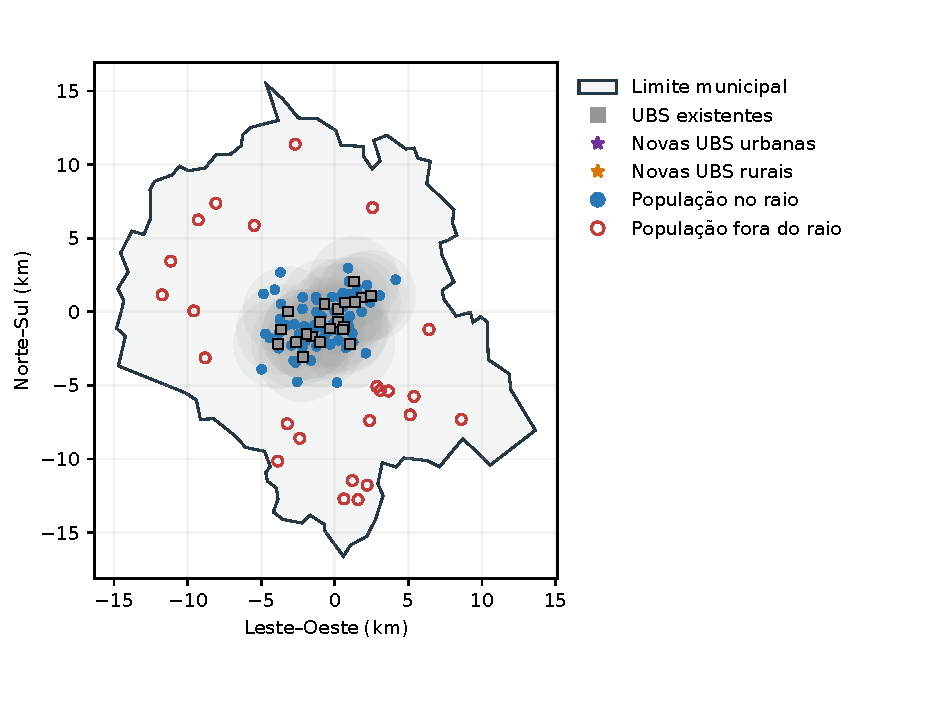
\includegraphics[width=.92\linewidth,height=.38\textheight,keepaspectratio]{figuras/mapa_rede_atual.pdf}
\caption{Rede atual com 22 UBS}\label{fig:mapa_atual}
\end{subfigure}

\vspace{10pt}
\begin{subfigure}{\linewidth}\centering
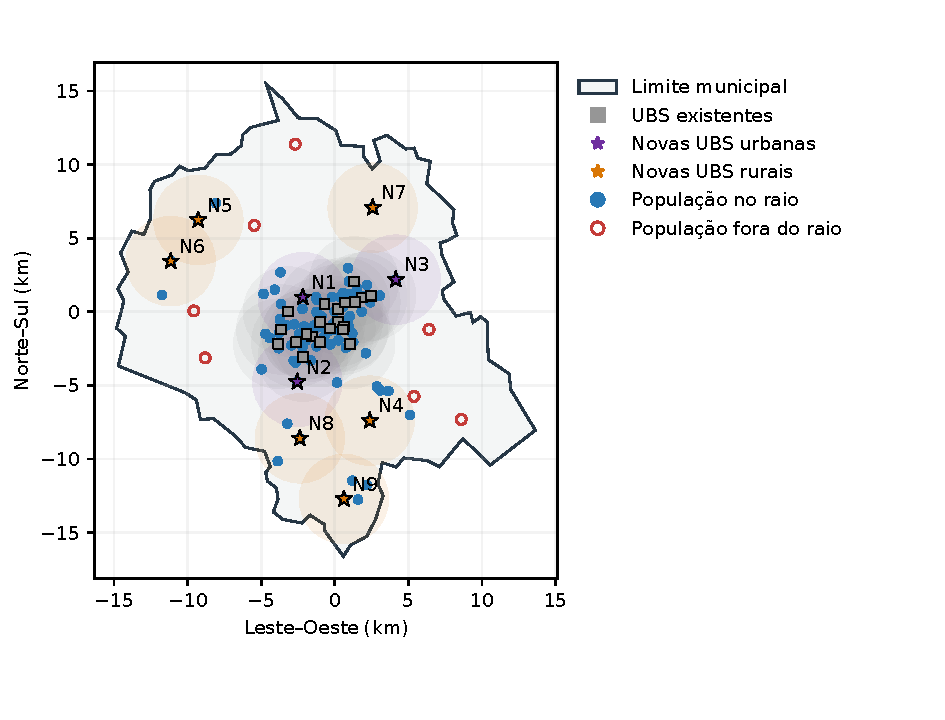
\includegraphics[width=.92\linewidth,height=.38\textheight,keepaspectratio]{figuras/mapa_plano_par.pdf}
\caption{Plano proposto com as 22 UBS existentes e as novas UBS N1 a N9}\label{fig:mapa_plano}
\end{subfigure}
\caption{Localização das UBS e cobertura geográfica no raio de 3 km, antes e depois do plano}\label{fig:mapa}
\fonte{Resultados do modelo, com dados de \citet{ibge2022} e \citet{cnes2026}.}
\nota{Códigos N1 a N9 conforme a Tabela~\ref{tab:unidades}. A base das equipes móveis (UBS Alto do Rosário)
não é representada.}
\end{figure}

A Figura~\ref{fig:acesso} mostra a população acumulada segundo a distância até a UBS mais próxima. Na
rede atual, os setores rurais mais afastados chegam a 10,4 km de uma UBS, e com as novas unidades a maior
distância cai para 7,0 km. Essa curva mede apenas a proximidade, sem levar em conta a capacidade das
equipes, que é o foco da comparação seguinte. A população que mora a mais de 3 km de uma UBS cai de
6.862 para 2.385 habitantes.

\begin{figure}[htbp]\centering
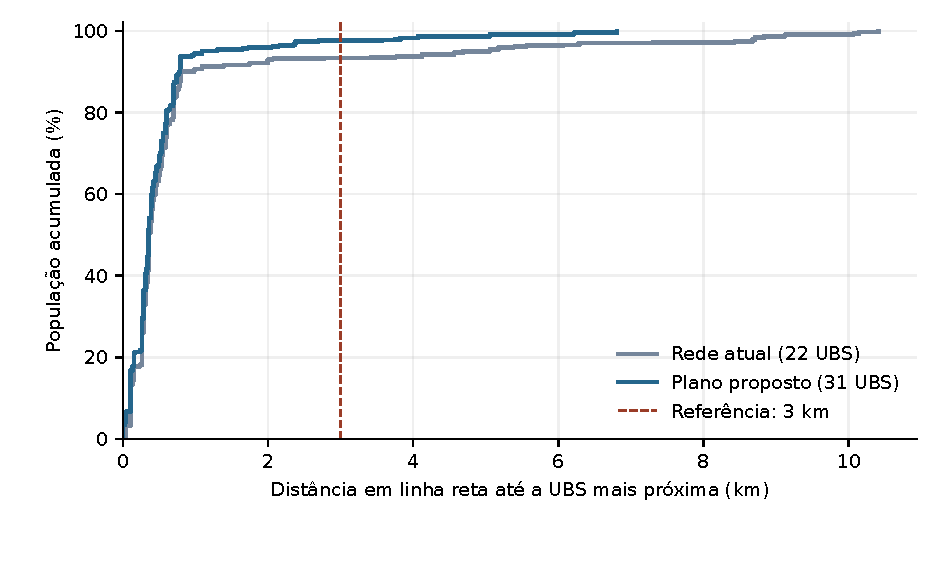
\includegraphics[width=.85\linewidth]{figuras/curva_acesso_geografico.pdf}
\caption{População acumulada segundo a distância até a UBS mais próxima, na rede atual e no plano proposto}\label{fig:acesso}
\fonte{Resultados do modelo de localização e dimensionamento.}
\end{figure}

O modelo nunca aloca a uma UBS mais pessoas do que as suas equipes comportam, e por isso a cobertura com
capacidade mede quantas pessoas podem de fato ser acompanhadas por uma equipe. Na rede atual, as 23 eSF
comportam 69.000 habitantes para uma população de 104.002. Com o limite dos ACS, a capacidade efetiva cai
para 68.250, e 35.752 pessoas ficam sem equipe disponível, o que explica a cobertura com capacidade de
65,6\%.

No plano, as 39 eSF comportam 117.000 habitantes. As UBS existentes continuam lotadas, e a expansão vem
das novas unidades. As urbanas atendem 28.560 habitantes, 95\% da capacidade das suas equipes, e as rurais
atendem 6.443, cerca de 36\%, pois cada uma tem uma eSF para 3.000 pessoas e atende entre 520 e 1.553. A
Tabela~\ref{tab:unidades} detalha esses valores por UBS, e a Figura~\ref{fig:utilizacao} mostra de forma
visual a ocupação de cada uma. Essa diferença entre unidades urbanas lotadas e
rurais ociosas é retomada na discussão.

\begin{table}[htbp]\centering\small\setlength{\tabcolsep}{3pt}
\caption{Unidades fixas, recursos planejados e ocupação}\label{tab:unidades}
\begin{tabular}{p{.39\linewidth}rrrrr}
\toprule Unidade & eSF & ACS & População & No raio & \shortstack{Ocupação\\(\%)}\\\midrule
\multicolumn{6}{l}{\textit{UBS existentes}}\\
UBS Alto do Rosário & 1 & 6 & 3.000 & 3.000 & 100\\
UBS Central & 1 & 5 & 3.000 & 3.000 & 100\\
UBS Cidade Nova & 1 & 9 & 3.000 & 3.000 & 100\\
UBS Garcias & 1 & 6 & 3.000 & 3.000 & 100\\
UBS Graças & 1 & 5 & 3.000 & 3.000 & 100\\
UBS Irmãos Auler & 1 & 6 & 3.000 & 3.000 & 100\\
UBS Itaunense & 1 & 5 & 3.000 & 3.000 & 100\\
UBS Jadir Marinho & 1 & 6 & 3.000 & 3.000 & 100\\
UBS Lourdes & 1 & 5 & 3.000 & 3.000 & 100\\
UBS Morada Nova & 1 & 4 & 3.000 & 3.000 & 100\\
UBS Morada Nova II & 1 & 6 & 3.000 & 3.000 & 100\\
UBS Morro do Engenho & 1 & 6 & 3.000 & 3.000 & 100\\
UBS Nogueira Machado & 1 & 6 & 3.000 & 3.000 & 100\\
UBS Padre Eustáquio & 1 & 6 & 3.000 & 3.000 & 100\\
UBS Parque Jardim Santanense / Residencial Santanense & 2 & 10 & 6.000 & 6.000 & 100\\
UBS Piedade & 1 & 6 & 3.000 & 3.000 & 100\\
UBS Pio XII & 1 & 6 & 3.000 & 3.000 & 100\\
UBS Santanense & 1 & 6 & 3.000 & 3.000 & 100\\
UBS São Geraldo & 1 & 7 & 3.000 & 3.000 & 100\\
UBS Várzea da Olaria & 1 & 6 & 3.000 & 3.000 & 100\\
UBS Vila Tavares & 1 & 6 & 3.000 & 3.000 & 100\\
UBS Zona Rural & 1 & 13 & 3.000 & 3.000 & 100\\
\midrule
\multicolumn{6}{l}{\textit{Novas UBS urbanas}}\\
Residencial Victor Gonçalves de Souza (N1) & 4 & 16 & 12.000 & 12.000 & 100\\
Setor 313380805000191 (N2) & 3 & 12 & 9.000 & 9.000 & 100\\
Setor 313380805000177 (N3) & 3 & 11 & 7.560 & 7.140 & 84\\
\midrule
\multicolumn{6}{l}{\textit{Novas UBS rurais}}\\
Setor 313380805000267 (N4) & 1 & 3 & 1.553 & 1.099 & 52\\
Setor 313380805000115 (N5) & 1 & 2 & 1.297 & 836 & 43\\
Setor 313380805000197 (N6) & 1 & 2 & 1.267 & 677 & 42\\
Setor 313380805000174 (N7) & 1 & 2 & 985 & 524 & 33\\
Setor 313380805000188 (N8) & 1 & 2 & 821 & 821 & 27\\
Setor 313380805000185 (N9) & 1 & 1 & 520 & 520 & 17\\
\midrule
Total & 39 & 192 & 104.002 & 101.617 & \\
\bottomrule\end{tabular}
\fonte{Resultados do modelo de localização e dimensionamento.}
\nota{Ocupação = população alocada / (3.000 $\times$ eSF).}
\end{table}

\begin{figure}[p]\centering
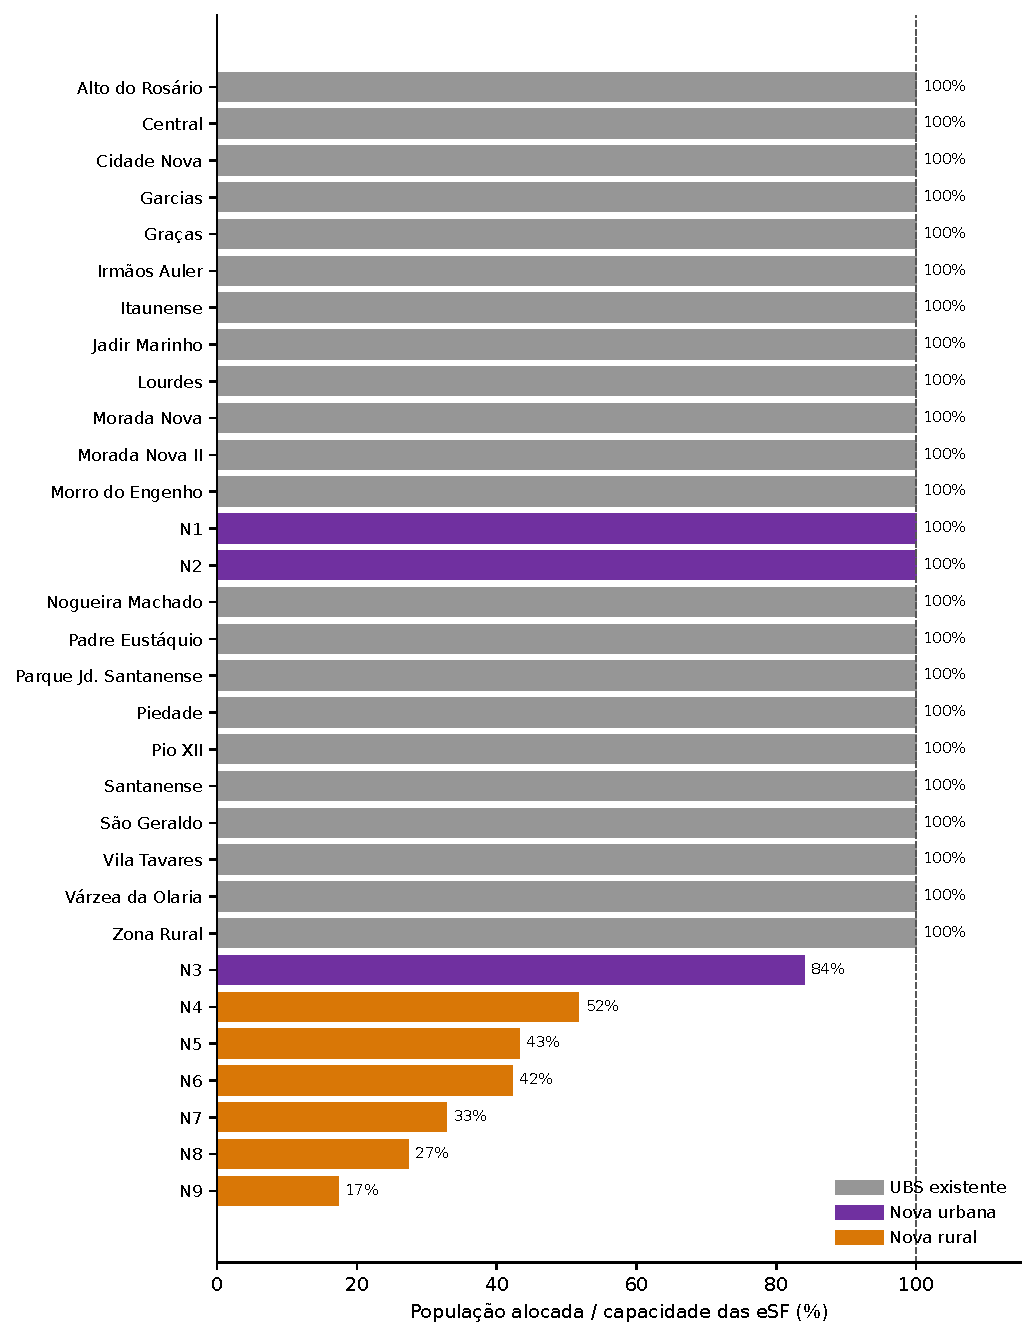
\includegraphics[width=.96\linewidth,height=.82\textheight,keepaspectratio]{figuras/ocupacao_equipes.pdf}
\caption{Ocupação das equipes fixas nas 31 UBS do plano, ordenada do maior para o menor percentual}\label{fig:utilizacao}
\fonte{Resultados do modelo de localização e dimensionamento.}
\nota{Ocupação = população alocada / (3.000 $\times$ eSF). As cores distinguem UBS existentes, novas urbanas e
novas rurais. N1 a N9 seguem a Tabela~\ref{tab:unidades}. As equipes móveis não entram no cálculo.}
\end{figure}

\begin{table}[htbp]\centering
\caption{Base do complemento móvel}\label{tab:movel}
\begin{tabular}{lrrr}\toprule UBS-base & Equipes & ACS & População atendida\\\midrule
UBS Alto do Rosário & 2 & 4 & 2.385,24\\
\bottomrule\end{tabular}
\fonte{Resultados do modelo do complemento móvel.}
\nota{Soluções com o mesmo número mínimo de equipes podem ter bases alternativas.}
\end{table}

\section{Funcionamento e investimento}

A Tabela~\ref{tab:custos} resume os custos estimados. O funcionamento da rede proposta custa
R\$ 3,00 milhões por mês, dos quais cerca de dois terços correspondem às 22 UBS existentes. A construção
das nove UBS soma R\$ 22,8 milhões, com R\$ 11,9 milhões nas seis rurais. A Tabela~\ref{tab:orcamento}
compara esses valores com a dotação de 2026. O funcionamento anual equivale a 70,7\% da dotação, contra
47,6\% da rede atual. A construção, por ser um investimento único, não entra nesses percentuais.

\begin{table}[htbp]\centering
\caption{Custos estimados da rede proposta}\label{tab:custos}
\begin{tabular}{lr}\toprule Componente & Valor (R\$)\\\midrule
UBS existentes (22), por mês & 2.024.060,25\\
UBS novas (9), por mês & 889.782,89\\
Pessoal das equipes móveis, por mês & 83.226,00\\
Funcionamento total, por mês & 2.997.069,14\\
Funcionamento total, por ano & 35.964.829,67\\
Construção das novas UBS (uma vez) & 22.848.000,00\\
\bottomrule\end{tabular}
\fonte{Resultados do modelo, com custos de referência descritos na Seção~\ref{sec:modeloaps} e \citet{novopac2025}.}
\nota{Veículos e combustível das equipes móveis, terrenos e equipamentos não foram precificados.}
\end{table}

\begin{table}[htbp]\centering
\caption{Custos estimados em relação à dotação atualizada da Atenção Básica de 2026}\label{tab:orcamento}
\begin{tabular}{lrr}\toprule Item & Valor anual (R\$) & \% da dotação\\\midrule
Dotação atualizada da Atenção Básica & 50.894.556,87 & 100,0\\
Rede atual, pessoal estimado e custos fixos & 24.232.528,33 & 47,6\\
Rede proposta, funcionamento & 35.964.829,67 & 70,7\\
\bottomrule\end{tabular}
\fonte{RREO, Anexo 02, quarto bimestre de 2026 \citep{tesouro2026}, e resultados do modelo.}
\nota{A dotação não é saldo livre, pois outras despesas da atenção primária não modeladas também a consomem.}
\end{table}

\section{Encaminhamentos especializados}\label{sec:encaminhamentos}

A Tabela~\ref{tab:ambulatorial} mostra os procedimentos alocados nos seis cenários, que combinam as duas
classificações com os três valores de $r$. A média complexidade é praticamente toda atendida em todos
eles. Na alta complexidade, a classificação única aloca 11.829 dos 15.863 procedimentos projetados, ou
74,6\%. A classificação de dois níveis eleva esse valor para 12.746, ou 80,3\%, e reduz a distância média
em cerca de 5\%. O volume de alta complexidade atendido não muda com $r$, e a média
complexidade só cai um pouco na classificação única com $r=75\%$.

\begin{table}[htbp]\centering
\caption{Procedimentos ambulatoriais alocados por cenário (procedimentos/ano)}\label{tab:ambulatorial}
\setlength{\tabcolsep}{5pt}
\begin{tabular}{llrrrr}\toprule
Classificação & Via sec. (\%) & Nível 2 & Nível 3 & Nível 3 atendido (\%) & Distância (km)\\\midrule
Única & 25 & 192.205,1 & 11.829,0 & 74,6 & 3,89\\
Única & 50 & 192.205,1 & 11.829,0 & 74,6 & 3,95\\
Única & 75 & 192.136,6 & 11.829,0 & 74,6 & 4,01\\
Dois níveis & 25 & 192.205,1 & 12.746,0 & 80,3 & 3,70\\
Dois níveis & 50 & 192.205,1 & 12.746,0 & 80,3 & 3,75\\
Dois níveis & 75 & 192.205,1 & 12.746,0 & 80,3 & 3,81\\
\bottomrule\end{tabular}
\fonte{Resultados do modelo de encaminhamento hierárquico.}
\nota{Distância média por percurso, em linha reta, ponderada pelos volumes atendidos. Como os volumes
alocados diferem entre cenários, as médias não se referem exatamente aos mesmos atendimentos.}
\end{table}

A Figura~\ref{fig:capacidades} explica a falta na alta complexidade. O hospital usa 38,1\% da sua
capacidade ambulatorial total, mas atinge 100\% do limite específico de alta complexidade, que não pode
ser ampliado com a capacidade que sobra. Os demais estabelecimentos atendem a média complexidade e
ficam no limite, exceto o centro de especialidades, que usa 72\% da sua capacidade.

\begin{figure}[htbp]\centering
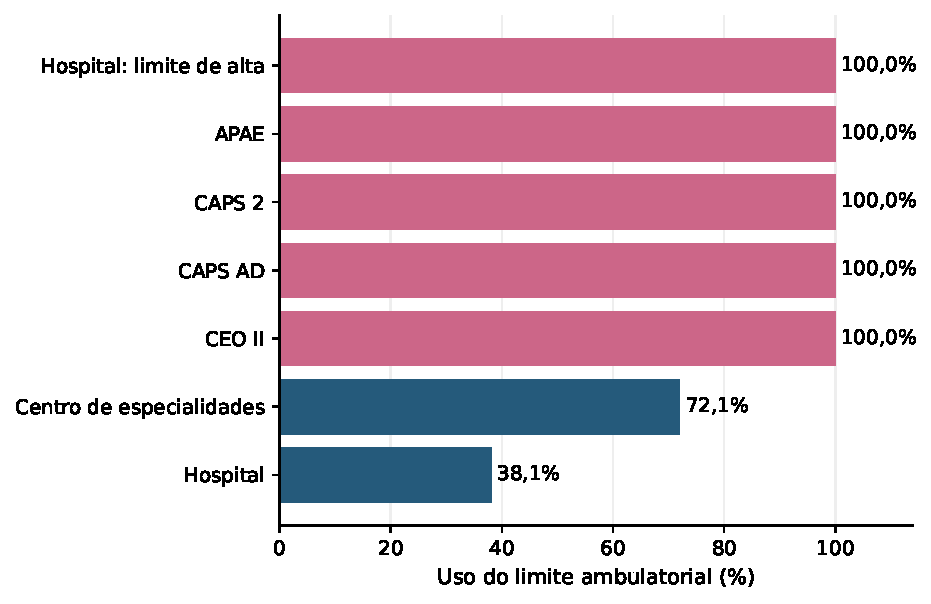
\includegraphics[width=.95\linewidth]{figuras/capacidades.pdf}
\caption{Uso dos limites ambulatoriais na classificação única, com 50\% via secundária, incluindo o limite
de alta complexidade do hospital}\label{fig:capacidades}
\fonte{Resultados do modelo de encaminhamento hierárquico.}
\end{figure}

As internações eletivas projetadas somam 1.072,5 de média e 352,5 de alta complexidade por ano e
exigiriam cerca de 6.676 dias-leito. No cenário conservador de leitos, nenhuma é alocada. No cenário
favorável, com 6.136 dias-leito, a classificação de dois níveis aloca 92,6\% das internações, enquanto a
classificação única aloca de 6\% a 19\% (Tabela~\ref{tab:leitos_otimista}). A diferença ocorre porque, na
classificação única, o hospital é apenas terciário e não recebe internações de média complexidade.

\begin{table}[htbp]\centering
\caption{Internações eletivas alocadas no cenário de disponibilidade hospitalar mais favorável}\label{tab:leitos_otimista}
\begin{tabular}{llrrr}\toprule Classificação & Via sec. (\%) & Média (\%) & Alta (\%) & Total (\%)\\\midrule
Única & 25 & 0,0 & 75,0 & 18,6\\
Única & 50 & 0,0 & 50,0 & 12,4\\
Única & 75 & 0,0 & 25,0 & 6,2\\
Dois níveis & 25 & 90,2 & 100,0 & 92,6\\
Dois níveis & 50 & 90,2 & 100,0 & 92,6\\
Dois níveis & 75 & 90,2 & 100,0 & 92,6\\
\bottomrule\end{tabular}
\fonte{Resultados do modelo de encaminhamento hierárquico com 6.136,35 dias-leito gerais.}
\nota{Percentual das internações/ano projetadas. O limite favorável é um extremo de sensibilidade, e não
capacidade residual observada. No cenário conservador, nenhuma internação é alocada.}
\end{table}

\section{Acessibilidade por zona}

A Tabela~\ref{tab:acessibilidade} mostra o índice de acessibilidade médio por zona, em valor absoluto e
relativo à média de cada rede. Na rede atual, o índice rural é 0,19 vez a média municipal com $\beta=1$ e
cai para 0,02 com $\beta=2$, que penaliza mais as distâncias longas. Na rede proposta, o índice rural
passa a superar a média, chegando a 1,10 com $\beta=1$, por causa das novas UBS rurais.

\begin{table}[htbp]\centering
\caption{Índice de acessibilidade médio por zona}\label{tab:acessibilidade}
\begin{tabular}{llrrr}\toprule Rede & Zona & $\beta$ & Índice absoluto & Índice relativo\\\midrule
Atual & Urbana & 1 & 0,689 & 1,04\\
Atual & Rural & 1 & 0,129 & 0,19\\
Atual & Urbana & 2 & 0,695 & 1,05\\
Atual & Rural & 2 & 0,013 & 0,02\\
Proposta & Urbana & 1 & 1,119 & 0,99\\
Proposta & Rural & 1 & 1,243 & 1,10\\
Proposta & Urbana & 2 & 1,006 & 0,89\\
Proposta & Rural & 2 & 3,583 & 3,19\\
\bottomrule\end{tabular}
\fonte{Resultados do diagnóstico de acessibilidade.}
\nota{A média municipal do índice absoluto é 0,663 na rede atual e 1,125 na proposta. O índice usa apenas as
eSF fixas e não é um percentual.}
\end{table}

\section{Sensibilidade}

A Tabela~\ref{tab:sensibilidade} altera um parâmetro de cada vez em relação ao cenário principal. A
curva de cobertura e custo, na Figura~\ref{fig:curva}, impõe metas mínimas de cobertura com capacidade, sem a folga de
2\%, e por isso o seu ponto de cobertura máxima custa um pouco menos que o cenário principal. O
custo inclui as equipes móveis necessárias para completar a cobertura. Com a meta de 93,4\%, são cinco
equipes móveis, o que torna esse ponto mais caro que o de 95\%. Metas acima de 97,7\% são inviáveis só
com UBS fixas.

A Figura~\ref{fig:investimento_cobertura} mostra, para os mesmos cenários, apenas o investimento em
construção. Cada ponto é um plano reotimizado para uma meta de cobertura, e o salto entre pontos mostra
quanto custa ampliar a meta. Para 93,4\% bastam três UBS urbanas. Cada meta acima disso exige
também unidades rurais, de uma em 95\% a seis em 97,7\%, e o investimento sobe até os R\$ 22,85 milhões
do cenário principal.

Um raio rural de 5 km reduz o número de UBS novas e eleva a cobertura rural de 53,5\% para 82,1\%, com
3 km na zona urbana, ou para 90,4\%, com 5 km nas duas zonas (Figura~\ref{fig:raios_cobertura}). Sem
mínimo de população rural, o plano abre 14 UBS, e com mínimo de 1.000 habitantes, apenas quatro. Com 5\%
e 10\% mais habitantes que em 2026, são necessárias 10 e 13 UBS novas. A folga de 5\% produz a mesma
solução do cenário principal.

\begin{table}[htbp]\centering\small
\caption{Sensibilidade do plano da atenção primária}\label{tab:sensibilidade}
\begin{tabular}{p{.36\linewidth}rrrrr}
\toprule Cenário & \shortstack{Novas\\UBS} & \shortstack{Cob.\\(\%)} & \shortstack{Equipes\\móveis} & \shortstack{Operação\\(mil R\$/mês)} & \shortstack{Construção\\(mi R\$)}\\\midrule
Principal (3 km, mínimo rural 500, folga 2\%) & 9 & 97,71 & 2 & 2.997,07 & 22,85\\
\midrule
\multicolumn{6}{l}{\textit{Curva de cobertura e custo (folga nula)}}\\
Cobertura mínima de 93,4\% & 3 & 93,40 & 5 & 2.888,87 & 12,92\\
Cobertura mínima de 95,0\% & 4 & 95,00 & 4 & 2.862,26 & 13,46\\
Cobertura mínima de 96,0\% & 5 & 96,00 & 4 & 2.863,21 & 14,90\\
Cobertura mínima de 97,0\% & 7 & 97,00 & 3 & 2.920,77 & 18,87\\
Cobertura máxima & 9 & 97,71 & 2 & 2.978,34 & 22,85\\
\midrule
\multicolumn{6}{l}{\textit{Raio de cobertura (urbano/rural)}}\\
2/2 km & 9 & 95,72 & 4 & 3.006,43 & 20,87\\
3/5 km & 8 & 99,03 & 1 & 2.912,89 & 20,86\\
5/5 km & 7 & 99,56 & 1 & 2.846,91 & 19,11\\
\midrule
\multicolumn{6}{l}{\textit{Mínimo de abertura rural}}\\
Sem mínimo & 14 & 99,86 & 1 & 3.191,69 & 32,79\\
1.000 habitantes & 4 & 94,81 & 4 & 2.866,94 & 13,46\\
\midrule
\multicolumn{6}{l}{\textit{Outros parâmetros}}\\
Folga operacional de 5\% & 9 & 97,71 & 2 & 2.997,07 & 22,85\\
População 5\% maior & 10 & 98,19 & 2 & 3.099,98 & 25,84\\
População 10\% maior & 13 & 99,07 & 1 & 3.279,18 & 32,12\\
\bottomrule\end{tabular}
\fonte{Resultados das análises de sensibilidade.}
\nota{Cob. é a cobertura com capacidade das UBS fixas, medida no raio de cada cenário, e por isso cenários
com raios diferentes não são diretamente comparáveis. A operação inclui as UBS e o pessoal das equipes
móveis. Metas de 98\%, 99\% e 99,5\% são inviáveis só com UBS fixas no raio de 3 km.}
\end{table}

\begin{figure}[htbp]\centering
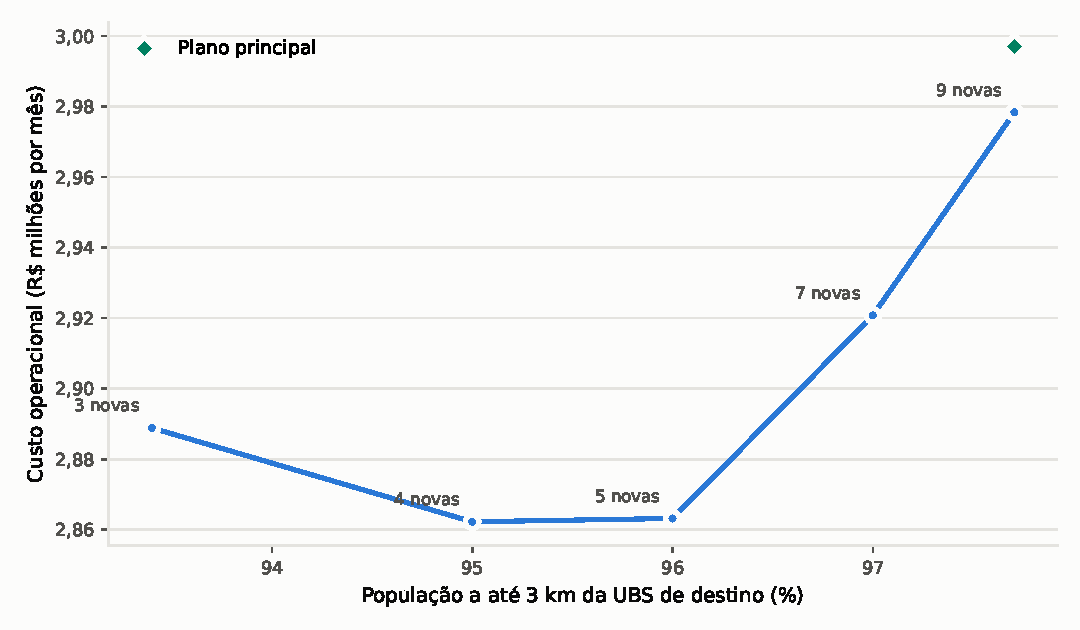
\includegraphics[width=.98\linewidth]{figuras/curva_cobertura_custo.pdf}
\caption{Custo operacional nos cenários de meta de cobertura com capacidade}\label{fig:curva}
\fonte{Resultados das análises de sensibilidade.}
\end{figure}

\begin{figure}[htbp]\centering
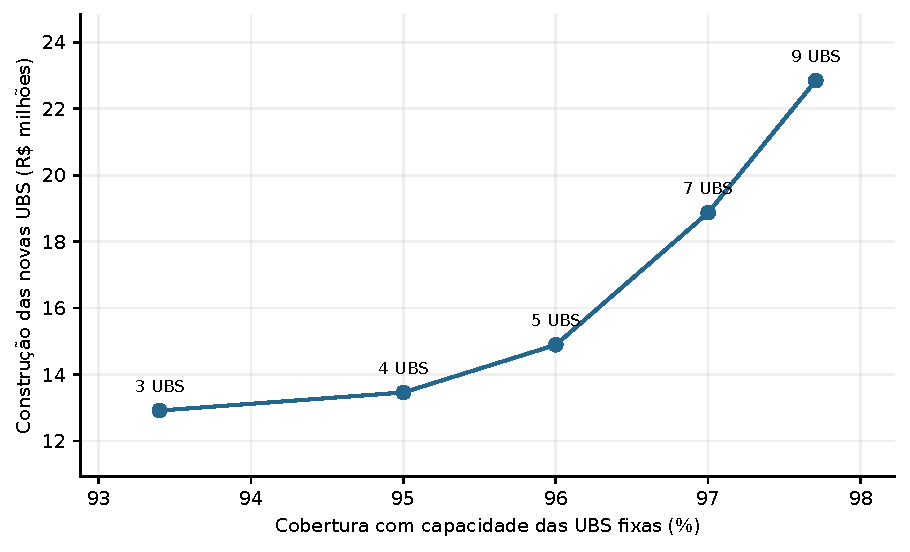
\includegraphics[width=.92\linewidth]{figuras/investimento_cobertura.pdf}
\caption{Investimento em construção nos cenários de meta de cobertura}\label{fig:investimento_cobertura}
\fonte{Resultados da análise de sensibilidade, com custos por porte do Novo PAC Saúde \citep{novopac2025}.}
\nota{Raio de 3 km e folga operacional nula. O eixo vertical inclui apenas a construção das UBS. Os rótulos
indicam quantas novas UBS cada plano abre.}
\end{figure}


\begin{figure}[htbp]\centering
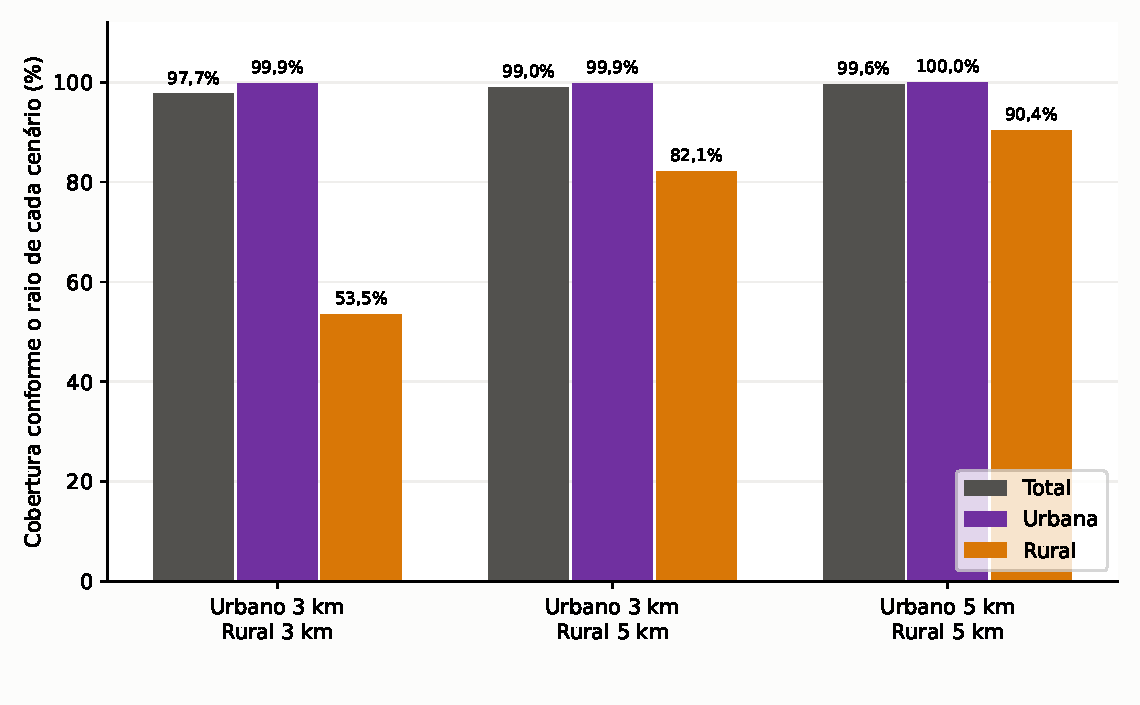
\includegraphics[width=.9\linewidth]{figuras/extra_raios_02_cobertura.pdf}
\caption{Cobertura total, urbana e rural nos cenários de raio}\label{fig:raios_cobertura}
\fonte{Resultados das análises de sensibilidade.}
\end{figure}


\section{Discussão}\label{sec:discussao}

\subsection{Expansão da atenção primária e custo da cobertura rural}
O principal resultado é que, com os parâmetros adotados, o maior déficit da atenção primária de Itaúna é de
capacidade. Quase toda a população mora a até 3 km de uma UBS, mas as equipes
existentes não comportam todos os moradores. A distância também pesa para os moradores mais afastados, e por
isso o plano amplia ainda a cobertura geográfica. É a situação de necessidade e demanda sem oferta suficiente
descrita por \citet{santana2023}, que ilustra a diferença entre proximidade e disponibilidade apontada por
\citet{guagliardo2004}. \citet{elorza2022} chegaram a conclusão semelhante em outra rede de atenção
primária, com unidades bem distribuídas e oferta insuficiente. Como as salas das UBS existentes não
comportam novas equipes, a expansão depende de novas unidades.

O investimento necessário para cada ponto percentual de cobertura cresce à medida que a meta sobe, como
na relação entre número de instalações e cobertura estudada por \citet{church1974}. Três UBS urbanas, com
R\$ 12,9 milhões de construção, já resolvem a maior parte do déficit de capacidade. Já os últimos 0,7
ponto percentual, de 97,0\% para 97,7\%, exigem mais duas UBS e cerca de R\$ 4 milhões, por causa das
unidades rurais. Cada UBS rural custa R\$ 1,99 milhão de construção e, em média, R\$ 57 mil por mês para
atender de 520 a 1.553 pessoas.

Esse é o conflito entre eficiência e equidade que \citet{ahmadi2017} apontam como central nos serviços
não emergenciais, e o desequilíbrio entre áreas urbanas e rurais motivou o modelo de \citet{hodgson1988}.
As UBS rurais aproximam o serviço de pequenos grupos dispersos, mas ficam com boa parte da capacidade
ociosa. Essa escolha atende à universalidade e à igualdade de acesso previstas para o SUS
\citep{brasil1988cf,brasil1990}, e o modelo mostra quanto ela custa. A sensibilidade aponta alternativas,
como exigir 1.000 habitantes para abrir uma UBS rural, com menos obras e mais equipes móveis, ou adotar
um raio rural de 5 km. A escolha entre elas é uma decisão de política de saúde.

O plano também aumenta a distância até a UBS de vínculo. A distância média passa de 0,85 km para 0,98 km,
e a população a até 1 km da sua UBS cai de 90,7\% para 65,5\%. A situação atual liga cada ponto à UBS
mais próxima, sem limite de capacidade, enquanto o plano respeita esse limite e transfere parte dos
moradores do centro para unidades novas, que precisam estar a mais de 1 km das existentes. Esse é o custo
em deslocamento de tornar a capacidade compatível com a população.

Essa transferência decorre da alocação múltipla, que não considera a preferência do usuário pela unidade
mais próxima \citep{contreras2019}. Na prática, parte dos moradores pode continuar procurando a UBS mais
próxima, embora \citet{hodgson1988} observe que a escolha do paciente nem sempre segue esse critério.
Exigir a alocação à unidade mais próxima tornaria o problema mais restrito e, com a capacidade limitada,
poderia exigir outra configuração da rede ou reduzir a cobertura.

\subsection{Rede especializada}
A falta na alta complexidade não significa necessariamente desassistência. A demanda foi estimada pela
produção dos moradores, que inclui atendimentos feitos em outros municípios, enquanto a oferta considera
apenas os estabelecimentos de Itaúna. O resultado indica, portanto, o volume que depende de referência a
outros municípios da região. Isso é coerente com o princípio de economia de escala das redes de atenção,
segundo o qual os serviços de alta complexidade se concentram em polos regionais
\citep{brasil2010,mendes2010}.

A classificação de dois níveis ilustra a oferta aninhada descrita por \citet{sahin2007}. O ganho de
atendimento é pequeno, pois o centro de especialidades produz pouca alta complexidade, e o ganho de
distância vem dos encaminhamentos entre níveis dentro do mesmo estabelecimento. Nas internações, a
variação entre zero e 92,6\% mostra que faltam dados de ocupação por tipo de leito, que também são a
base dos parâmetros hospitalares do SUS \citep{brasil2015b}. Com esses dados, o modelo poderia estimar a
capacidade real, como fazem \citet{guerriero2016} ao usar a ocupação e a permanência média para
reorganizar uma rede hospitalar.

\subsection{Implicações orçamentárias}
O funcionamento da rede proposta custa R\$ 35,96 milhões por ano, 70,7\% da dotação atualizada da
Atenção Básica, contra R\$ 24,23 milhões, ou 47,6\%, da rede atual (Tabela~\ref{tab:orcamento}). O
acréscimo de R\$ 11,73 milhões, que já inclui o pessoal das equipes móveis, equivale a 23,1\% da dotação.
Como a dotação também financia despesas que não entram no modelo, esses percentuais mostram o peso do
plano no orçamento, e não uma folga disponível.

A construção das nove UBS, de R\$ 22,85 milhões, é um investimento único e foi tratada à parte, pois
recursos de capital e de custeio costumam ter fontes e prazos diferentes. O Novo PAC Saúde é uma possível
fonte federal para as obras, mas depende de seleção e habilitação das propostas
\citep{pacselecao2025,novopac2025}. Uma implantação em etapas distribuiria o investimento entre
exercícios, e o funcionamento cresceria à medida que cada unidade entrasse em operação. A
Figura~\ref{fig:investimento_cobertura} sugere uma ordem, começando pelas UBS urbanas, que resolvem a
maior parte do déficit com menor investimento.

\section{Limitações e trabalhos futuros}
Os resultados dependem de simplificações que indicam os próximos passos do estudo. A demanda
especializada vem da utilização registrada, o que dimensiona a rede para o padrão atual de atendimento,
mas não capta filas e demanda reprimida \citep{santana2023}, e usa uma taxa única por habitante, sem
ajuste por idade ou risco. Os 91 pontos aproximam o território, as candidatas não são terrenos
confirmados e as distâncias são em linha reta, embora a acessibilidade dependa do tempo de viagem
efetivo \citep{aday1974}.

Na rede especializada, a agregação por nível não verifica a compatibilidade entre especialidades, e as
parcelas $r$ são cenários, e não estimativas feitas com dados de encaminhamento. A capacidade
ambulatorial vem do mês de maior produção, que pode não se manter ao longo do ano. Nas internações, não
se sabe quanto dos leitos gerais é ocupado por urgências e outros atendimentos, o que explica a grande
diferença entre os cenários hospitalares. Além disso, uma internação pode reunir procedimentos de
complexidades diferentes, e por isso os fluxos entre níveis não devem ser lidos como transferências.

Nos custos, os salários são valores de referência, e não a folha do município, o custo fixo é o mesmo
para qualquer porte, e os veículos e o combustível das equipes móveis não foram incluídos. Essas equipes
também dependem de uma programação de visitas que não foi modelada. Por fim, a abordagem sequencial fixa a
atenção primária antes dos encaminhamentos e não garante o ótimo conjunto da rede, embora os níveis de
atenção sejam interdependentes \citep{hodgson1988}. Demanda e capacidade também foram tratadas como
valores conhecidos, e a otimização robusta ou a programação estocástica permitiriam avaliar o plano em
diferentes cenários \citep{snyder2006}.

% =====================================================================
\chapter{Conclusões}
Este trabalho combinou um modelo de localização com capacidade e um modelo de encaminhamento hierárquico
para planejar a rede de saúde de Itaúna. O principal resultado é que o maior déficit da atenção primária está
na capacidade das equipes, embora a distância também limite o acesso. Hoje, 93,4\% da população mora a até 3 km de
uma UBS, mas as equipes comportam apenas 65,6\% dos moradores dentro desse raio, e cerca de 35,8 mil
pessoas ficam sem equipe disponível. Outros 6,9 mil moradores estão a mais de 3 km de uma UBS.

O plano abre nove UBS e eleva a rede a 39 eSF e 192 ACS, com cobertura geográfica e com capacidade de 97,7\%, e duas
equipes móveis atendem os pontos mais distantes, o que leva a cobertura potencial a 100\%. O funcionamento custa R\$ 3,00 milhões por mês, 70,7\% da
dotação da Atenção Básica, e a construção exige R\$ 22,8 milhões, que podem ser distribuídos em etapas. As
UBS rurais são a parte mais cara em relação à população atendida, e a escolha entre elas, equipes móveis
ou um raio maior é uma decisão de equidade.

Na rede especializada, a média complexidade ambulatorial é quase toda atendida no município, mas cerca de
um quarto da alta complexidade depende de outros municípios. Oferecer dois níveis no hospital e no centro
de especialidades reduz essa parcela e a distância percorrida. As internações não puderam ser avaliadas
com precisão, pois faltam dados de ocupação dos leitos, e o resultado varia de nenhuma a 92,6\% das
internações atendidas conforme a hipótese adotada.

A aplicação do plano exige confirmar os terrenos, programar as visitas das equipes móveis e levantar a
ocupação dos leitos. Trabalhos futuros podem incluir a demanda reprimida, a estrutura etária, os tempos de
viagem pela malha viária, a alocação à UBS mais próxima e a incerteza da demanda \citep{snyder2006}. Um
modelo que decida ao mesmo tempo a expansão da atenção primária e os encaminhamentos permitiria avaliar a
rede como um todo.


% =====================================================================
\begin{thebibliography}{99}

\bibitem[Aday e Andersen(1974)]{aday1974}
ADAY, L. A.; ANDERSEN, R. A framework for the study of access to medical care. \textit{Health Services Research}, v. 9, n. 3, p. 208--220, 1974. Disponível em: \url{https://pubmed.ncbi.nlm.nih.gov/4436074/}. Acesso em: 10 nov. 2026.

\bibitem[Ahmadi-Javid et al.(2017)]{ahmadi2017}
AHMADI-JAVID, A.; SEYEDI, P.; SYAM, S. S. A survey of healthcare facility location. \textit{Computers \& Operations Research}, v. 79, p. 223--263, 2017. DOI: \url{https://doi.org/10.1016/j.cor.2016.05.018}.

\bibitem[Brasil(1962)]{brasil1962decimo}
BRASIL. Lei nº 4.090, de 13 de julho de 1962. Institui a gratificação de Natal para os trabalhadores. Brasília, DF, 1962. Disponível em: \url{https://www.planalto.gov.br/ccivil_03/leis/l4090.htm}. Acesso em: 25 nov. 2026.

\bibitem[Brasil(1988)]{brasil1988cf}
BRASIL. \textit{Constituição da República Federativa do Brasil de 1988}. Arts. 7º, XVII, e 196. Brasília, DF, 1988. Disponível em: \url{https://www.planalto.gov.br/ccivil_03/constituicao/constituicao.htm}. Acesso em: 25 nov. 2026.

\bibitem[Brasil(1990b)]{brasil1990fgts}
BRASIL. Lei nº 8.036, de 11 de maio de 1990. Dispõe sobre o Fundo de Garantia do Tempo de Serviço. Art. 15. Brasília, DF, 1990b. Disponível em: \url{https://www.planalto.gov.br/ccivil_03/leis/l8036compilada.htm}. Acesso em: 25 nov. 2026.

\bibitem[Brasil(1991)]{brasil1991custeio}
BRASIL. Lei nº 8.212, de 24 de julho de 1991. Dispõe sobre a organização da Seguridade Social e institui Plano de Custeio. Art. 22. Brasília, DF, 1991. Disponível em: \url{https://www.planalto.gov.br/ccivil_03/leis/l8212cons.htm}. Acesso em: 25 nov. 2026.

\bibitem[Brasil(1990a)]{brasil1990}
BRASIL. Lei nº 8.080, de 19 de setembro de 1990. Dispõe sobre as condições para a promoção, proteção e recuperação da saúde, a organização e o funcionamento dos serviços correspondentes e dá outras providências. Brasília, DF, 1990. Disponível em: \url{https://www.planalto.gov.br/ccivil_03/leis/l8080.htm}. Acesso em: 25 nov. 2026.

\bibitem[Brasil(2010)]{brasil2010}
BRASIL. Ministério da Saúde. Portaria nº 4.279, de 30 de dezembro de 2010. Estabelece diretrizes para a organização da Rede de Atenção à Saúde no âmbito do Sistema Único de Saúde (SUS). Brasília, DF, 2010. Disponível em: \url{https://bvsms.saude.gov.br/bvs/saudelegis/gm/2010/prt4279_30_12_2010.html}. Acesso em: 25 nov. 2026.

\bibitem[Brasil(2011)]{brasil2011}
BRASIL. Decreto nº 7.508, de 28 de junho de 2011. Regulamenta a Lei nº 8.080, de 19 de setembro de 1990, para dispor sobre a organização do Sistema Único de Saúde --- SUS, o planejamento da saúde, a assistência à saúde e a articulação interfederativa, e dá outras providências. Brasília, DF, 2011. Disponível em: \url{https://www.planalto.gov.br/ccivil_03/_ato2011-2014/2011/decreto/d7508.htm}. Acesso em: 24 nov. 2026.

\bibitem[Brasil(2015a)]{brasil2015a}
BRASIL. Ministério da Saúde. Portaria nº 1.631, de 1º de outubro de 2015. Aprova critérios e parâmetros para o planejamento e programação de ações e serviços de saúde no âmbito do SUS. Brasília, DF, 2015a. Disponível em: \url{https://bvsms.saude.gov.br/bvs/saudelegis/gm/2015/prt1631_01_10_2015.html}. Acesso em: 10 nov. 2026.

\bibitem[Brasil(2015b)]{brasil2015b}
BRASIL. Ministério da Saúde. Secretaria de Atenção à Saúde. \textit{Critérios e parâmetros para o planejamento e programação de ações e serviços de saúde no âmbito do Sistema Único de Saúde}. Brasília, DF: Ministério da Saúde, 2015b. (Série Parâmetros SUS, v. 1). Disponível em: \url{https://fehosp.com.br/files/manuais/5ffa8d1e03f7edb01e1eed7b07178cfb.pdf}. Acesso em: 10 nov. 2026.

\bibitem[Brasil(2013)]{brasil2013teto}
BRASIL. Ministério da Saúde. Portaria nº 2.355, de 10 de outubro de 2013. Altera a fórmula de cálculo do teto máximo das Equipes de Saúde da Família. Brasília, DF, 2013. Disponível em: \url{https://www.saude.mt.gov.br/storage/old/files/2355-[9229-191213-SES-MT].pdf}. Acesso em: 25 nov. 2026.

\bibitem[Brasil(2017)]{pnab2017}
BRASIL. Ministério da Saúde. Portaria nº 2.436, de 21 de setembro de 2017. Aprova a Política Nacional de Atenção Básica. Brasília, DF, 2017. Disponível em: \url{https://bvsms.saude.gov.br/bvs/saudelegis/gm/2017/prt2436_22_09_2017.html}. Acesso em: 10 nov. 2026.

\bibitem[Brasil(2022a)]{brasil2022}
BRASIL. Emenda Constitucional nº 120, de 5 de maio de 2022. Acrescenta §§ 7º, 8º, 9º, 10 e 11 ao art. 198 da Constituição Federal, para dispor sobre a responsabilidade financeira da União, corresponsável pelo SUS, na política remuneratória e na valorização dos profissionais que exercem atividades de agente comunitário de saúde e de agente de combate às endemias. Brasília, DF, 2022a. Disponível em: \url{https://www.planalto.gov.br/ccivil_03/constituicao/emendas/emc/emc120.htm}. Acesso em: 15 nov. 2026.

\bibitem[Brasil(2022b)]{brasil2022piso}
BRASIL. Lei nº 14.434, de 4 de agosto de 2022. Altera a Lei nº 7.498, de 25 de junho de 1986, para instituir o piso salarial nacional do Enfermeiro, do Técnico de Enfermagem, do Auxiliar de Enfermagem e da Parteira. Brasília, DF, 2022b. Disponível em: \url{https://www.planalto.gov.br/ccivil_03/_ato2019-2022/2022/lei/l14434.htm}. Acesso em: 25 nov. 2026.

\bibitem[Brasil(2026f)]{maismedicos2026}
BRASIL. Ministério da Saúde. Portaria SGTES/MS nº 211, de 5 de março de 2026. Dispõe sobre o valor da bolsa-formação paga aos médicos participantes do Projeto Mais Médicos para o Brasil. \textit{Diário Oficial da União}, Brasília, DF, 6 mar. 2026f. Disponível em: \url{https://www.legisweb.com.br/legislacao/?id=491990}. Acesso em: 25 nov. 2026.

\bibitem[Brasil(2025a)]{brasil2025sm}
BRASIL. Decreto nº 12.797, de 23 de dezembro de 2025. Dispõe sobre o valor do salário mínimo a vigorar a partir de 1º de janeiro de 2026. \textit{Diário Oficial da União}, Brasília, DF, 24 dez. 2025a. Disponível em: \url{https://www.planalto.gov.br/ccivil_03/_ato2023-2026/2025/decreto/d12797.htm}. Acesso em: 25 nov. 2026.

\bibitem[Brasil(2025b)]{novopac2025}
BRASIL. Ministério da Saúde. \textit{Manual de formalização de propostas}: Novo PAC Saúde. Brasília, DF: Ministério da Saúde, 2025b. Disponível em: \url{https://www.gov.br/saude/pt-br/centrais-de-conteudo/publicacoes/guias-e-manuais/2025/manual-de-formalizacao-de-propostas-novo-pac-saude.pdf}. Acesso em: 11 nov. 2026.

\bibitem[Brasil(2025c)]{pacselecao2025}
BRASIL. Ministério da Saúde. Portaria GM/MS nº 6.640, de 20 de fevereiro de 2025. Institui o PAC Seleções -- Saúde 2025. Brasília, DF, 2025c. Disponível em: \url{https://bvsms.saude.gov.br/bvs/saudelegis/gm/2025/prt6640_20_02_2025.html}. Acesso em: 25 nov. 2026.

\bibitem[Brasil(2026a)]{cnes2026}
BRASIL. Ministério da Saúde. \textit{Cadastro Nacional de Estabelecimentos de Saúde --- CNES}. Brasília, DF: Ministério da Saúde, 2026a. Competência: julho de 2026. Disponível em: \url{https://cnes.datasus.gov.br/}. Acesso em: 10 nov. 2026.

\bibitem[Brasil(2026b)]{datasus2026}
BRASIL. Ministério da Saúde. DATASUS. \textit{Transferência de arquivos dos sistemas SIA/SUS e SIH/SUS}. Brasília, DF: Ministério da Saúde, 2026b. Produção processada em 2025. Disponível em: \url{https://datasus.saude.gov.br/transferencia-de-arquivos/}. Acesso em: 10 nov. 2026.

\bibitem[Brasil(2026c)]{aps2026}
BRASIL. Ministério da Saúde. \textit{Relatórios Públicos da APS}: cobertura potencial estimada da Atenção Primária à Saúde. Brasília, DF, 2026c. Município: Itaúna, código 313380; competência julho de 2026. Disponível em: \url{https://relatorioaps.saude.gov.br/cobertura/aps}. Acesso em: 10 nov. 2026.

\bibitem[Brasil(2026d)]{tabnet}
BRASIL. Ministério da Saúde. DATASUS. \textit{Informações de Saúde (TABNET)}. Brasília, DF, 2026d. Disponível em: \url{https://datasus.saude.gov.br/informacoes-de-saude-tabnet/}. Acesso em: 10 nov. 2026.

\bibitem[Brasil(2026e)]{siops}
BRASIL. Ministério da Saúde. \textit{Sistema de Informações sobre Orçamentos Públicos em Saúde --- SIOPS}. Brasília, DF, 2026e. Itaúna, 2025, subfunção 301. Disponível em: \url{https://www.gov.br/saude/pt-br/acesso-a-informacao/siops}. Acesso em: 10 nov. 2026.

\bibitem[Brasil(s.d.)]{sigtap}
BRASIL. Ministério da Saúde. \textit{SIGTAP}: Sistema de Gerenciamento da Tabela de Procedimentos, Medicamentos e OPM do SUS. Brasília, DF, [s.d.]. Disponível em: \url{http://sigtap.datasus.gov.br/tabela-unificada/app/sec/inicio.jsp}. Acesso em: 10 nov. 2026.

\bibitem[Castro et al.(2019)]{castro2019}
CASTRO, M. C.; MASSUDA, A.; ALMEIDA, G.; MENEZES-FILHO, N. A.; ANDRADE, M. V.; NORONHA, K. V. M. S.; ROCHA, R.; MACINKO, J.; HONE, T.; TASCA, R. et al. Brazil's unified health system: the first 30 years and prospects for the future. \textit{The Lancet}, v. 394, n. 10195, p. 345--356, 2019.

\bibitem[Church e ReVelle(1974)]{church1974}
CHURCH, R.; REVELLE, C. The maximal covering location problem. \textit{Papers of the Regional Science Association}, v. 32, n. 1, p. 101--118, 1974. DOI: \url{https://doi.org/10.1007/BF01942293}.

\bibitem[Contreras e Ortiz-Astorquiza(2019)]{contreras2019}
CONTRERAS, I.; ORTIZ-ASTORQUIZA, C. Hierarchical facility location problems. In: LAPORTE, G.; NICKEL, S.; SALDANHA DA GAMA, F. (ed.). \textit{Location science}. 2. ed. Cham: Springer, 2019. p. 365--389. DOI: \url{https://doi.org/10.1007/978-3-030-32177-2_13}.

\bibitem[Daskin(2008)]{daskin2008}
DASKIN, M. S. What you should know about location modeling. \textit{Naval Research Logistics}, v. 55, n. 4, p. 283--294, 2008. DOI: \url{https://doi.org/10.1002/nav.20284}.

\bibitem[Daskin e Dean(2004)]{daskin2004}
DASKIN, M. S.; DEAN, L. K. Location of health care facilities. In: BRANDEAU, M. L.; SAINFORT, F.; PIERSKALLA, W. P. (ed.). \textit{Operations research and health care}: a handbook of methods and applications. Boston: Kluwer Academic, 2004. p. 43--76. DOI: \url{https://doi.org/10.1007/1-4020-8066-2_3}.

\bibitem[Ehrgott(2005)]{ehrgott2005}
EHRGOTT, M. \textit{Multicriteria optimization}. 2. ed. Berlin: Springer, 2005. DOI: \url{https://doi.org/10.1007/3-540-27659-9}.

\bibitem[Elorza et al.(2022)]{elorza2022}
ELORZA, M. E.; MOSCOSO, N. S.; BLANCO, A. M. Assessing performance in health care: a mathematical programming approach for the re-design of primary health care networks. \textit{Socio-Economic Planning Sciences}, v. 84, artigo 101454, 2022.

\bibitem[Freire et al.(2021)]{freire2021}
FREIRE, D. E. W. G.; FREIRE, A. R.; LUCENA, E. H. G.; CAVALCANTI, Y. W. A PNAB 2017 e o número de agentes comunitários de saúde na atenção primária do Brasil. \textit{Revista de Saúde Pública}, v. 55, artigo 85, 2021.

\bibitem[Guagliardo(2004)]{guagliardo2004}
GUAGLIARDO, M. F. Spatial accessibility of primary care: concepts, methods and challenges. \textit{International Journal of Health Geographics}, v. 3, artigo 3, 2004. DOI: \url{https://doi.org/10.1186/1476-072X-3-3}.

\bibitem[Guerriero et al.(2016)]{guerriero2016}
GUERRIERO, F.; MIGLIONICO, G.; OLIVITO, F. Location and reorganization problems: the Calabrian health care system case. \textit{European Journal of Operational Research}, v. 250, n. 3, p. 939--954, 2016.

\bibitem[Hakimi(1964)]{hakimi1964}
HAKIMI, S. L. Optimum locations of switching centers and the absolute centers and medians of a graph. \textit{Operations Research}, v. 12, n. 3, p. 450--459, 1964. DOI: \url{https://doi.org/10.1287/opre.12.3.450}.

\bibitem[Hansen(1959)]{hansen1959}
HANSEN, W. G. How accessibility shapes land use. \textit{Journal of the American Institute of Planners}, v. 25, n. 2, p. 73--76, 1959.

\bibitem[Hodgson(1988)]{hodgson1988}
HODGSON, M. J. An hierarchical location-allocation model for primary health care delivery in a developing area. \textit{Social Science \& Medicine}, v. 26, n. 1, p. 153--161, 1988.

\bibitem[Huangfu e Hall(2018)]{huangfu2018}
HUANGFU, Q.; HALL, J. A. J. Parallelizing the dual revised simplex method. \textit{Mathematical Programming Computation}, v. 10, n. 1, p. 119--142, 2018. DOI: \url{https://doi.org/10.1007/s12532-017-0130-5}.

\bibitem[IBGE(2022)]{ibge2022}
IBGE. Instituto Brasileiro de Geografia e Estatística. \textit{Censo Demográfico 2022}: agregados por setores censitários e resultados de população. Rio de Janeiro: IBGE, 2022. Disponível em: \url{https://www.ibge.gov.br/estatisticas/sociais/populacao/22827-censo-demografico-2022.html}. Acesso em: 10 nov. 2026.

\bibitem[IBGE(2025)]{ibge2025est}
IBGE. Instituto Brasileiro de Geografia e Estatística. \textit{Estimativas da população residente nos municípios brasileiros}: 2025. Rio de Janeiro: IBGE, 2025. Disponível em: \url{https://ftp.ibge.gov.br/Estimativas_de_Populacao/Estimativas_2025/POP2025_20251031.pdf}. Acesso em: 17 nov. 2026.

\bibitem[IBGE(2026)]{ibge2026est}
IBGE. Instituto Brasileiro de Geografia e Estatística. \textit{Estimativas da população residente nos municípios brasileiros}: 2026. Rio de Janeiro: IBGE, 2026. Disponível em: \url{https://ftp.ibge.gov.br/Estimativas_de_Populacao/Estimativas_2026/POP2026_20261029.pdf}. Acesso em: 17 nov. 2026.

\bibitem[Itaúna(2025)]{itauna2025}
ITAÚNA. Lei nº 6.273, de 30 de dezembro de 2025. Estima a receita e fixa a despesa do Município de Itaúna para o exercício de 2026 e dá outras providências. \textit{Jornal Oficial do Município de Itaúna}, n. 2.623, 30 dez. 2025. Disponível em: \url{https://sapl.itauna.mg.leg.br/media/sapl/public/normajuridica/2025/11182/lei_6273-2026_-_loa_2026.pdf}. Acesso em: 11 nov. 2026.

\bibitem[Joseph e Bantock(1982)]{joseph1982}
JOSEPH, A. E.; BANTOCK, P. R. Measuring potential physical accessibility to general practitioners in rural areas: a method and case study. \textit{Social Science \& Medicine}, v. 16, n. 1, p. 85--90, 1982. DOI: \url{https://doi.org/10.1016/0277-9536(82)90428-2}.

\bibitem[Makhorin(2008)]{glpk}
MAKHORIN, A. \textit{GLPK (GNU Linear Programming Kit)}. 2008. Disponível em: \url{http://www.gnu.org/s/glpk/glpk.html}. Acesso em: 25 nov. 2026.

\bibitem[Mendes(2010)]{mendes2010}
MENDES, E. V. As redes de atenção à saúde. \textit{Ciência \& Saúde Coletiva}, v. 15, n. 5, p. 2297--2305, 2010.

\bibitem[Mi\c{c} et al.(2019)]{mic2019}
MI\c{C}, P.; KOYUNCU, M.; HALLAK, J. Primary health care center (PHCC) location-allocation with multi-objective modelling: a case study in Idleb, Syria. \textit{International Journal of Environmental Research and Public Health}, v. 16, n. 5, artigo 811, 2019.

\bibitem[Mitchell et al.(2011)]{mitchell2011}
MITCHELL, S.; O'SULLIVAN, M.; DUNNING, I. \textit{PuLP}: a linear programming toolkit for Python. Auckland: The University of Auckland, 2011. Disponível em: \url{https://optimization-online.org/2011/09/3178/}. Acesso em: 24 nov. 2026.

\bibitem[Narula(1986)]{narula1986}
NARULA, S. C. Minisum hierarchical location-allocation problems on a network: a survey. \textit{Annals of Operations Research}, v. 6, p. 255--272, 1986.

\bibitem[Paim et al.(2011)]{paim2011}
PAIM, J.; TRAVASSOS, C.; ALMEIDA, C.; BAHIA, L.; MACINKO, J. The Brazilian health system: history, advances, and challenges. \textit{The Lancet}, v. 377, n. 9779, p. 1778--1797, 2011.

\bibitem[Rahman e Smith(2000)]{rahman2000}
RAHMAN, S.; SMITH, D. K. Use of location-allocation models in health service development planning in developing nations. \textit{European Journal of Operational Research}, v. 123, n. 3, p. 437--452, 2000. DOI: \url{https://doi.org/10.1016/S0377-2217(99)00289-1}.

\bibitem[Rodriguez Santana et al.(2023)]{santana2023}
RODRIGUEZ SANTANA, I.; MASON, A.; GUTACKER, N.; KASTERIDIS, P.; SANTOS, R.; RICE, N. Need, demand, supply in health care: working definitions, and their implications for defining access. \textit{Health Economics, Policy and Law}, v. 18, n. 1, p. 1--13, 2023. DOI: \url{https://doi.org/10.1017/S1744133121000293}.

\bibitem[\c{S}ahin e Süral(2007)]{sahin2007}
\c{S}AH\.{I}N, G.; SÜRAL, H. A review of hierarchical facility location models. \textit{Computers \& Operations Research}, v. 34, n. 8, p. 2310--2331, 2007. DOI: \url{https://doi.org/10.1016/j.cor.2005.09.005}.

\bibitem[Schultz(1970)]{schultz1970}
SCHULTZ, G. P. The logic of health care facility planning. \textit{Socio-Economic Planning Sciences}, v. 4, n. 3, p. 383--393, 1970.

\bibitem[Shengelia et al.(2005)]{shengelia2005}
SHENGELIA, B.; TANDON, A.; ADAMS, O. B.; MURRAY, C. J. L. Access, utilization, quality, and effective coverage: an integrated conceptual framework and measurement strategy. \textit{Social Science \& Medicine}, v. 61, n. 1, p. 97--109, 2005. DOI: \url{https://doi.org/10.1016/j.socscimed.2004.11.055}.

\bibitem[Snyder(2006)]{snyder2006}
SNYDER, L. V. Facility location under uncertainty: a review. \textit{IIE Transactions}, v. 38, n. 7, p. 547--564, 2006.

\bibitem[Tesouro Nacional(2026)]{tesouro2026}
TESOURO NACIONAL. \textit{Sistema de Informações Contábeis e Fiscais do Setor Público Brasileiro --- Siconfi}: Relatório Resumido da Execução Orçamentária, Anexo 02, 4º bimestre de 2026. Ente: Prefeitura Municipal de Itaúna, código IBGE 3133808. Disponível em: \url{https://apidatalake.tesouro.gov.br/ords/siconfi/tt/rreo?an_exercicio=2026&nr_periodo=4&co_tipo_demonstrativo=RREO&no_anexo=RREO-Anexo+02&id_ente=3133808}. Acesso em: 11 nov. 2026.

\end{thebibliography}

\appendix
\chapter{Fontes, rastreabilidade e reprodução}\label{ap:reproducao}

\section{Origem e transformação dos dados}
O estudo combina três tipos de dados. O CNES informa os recursos cadastrados, como equipes, salas e
leitos, o SIA e o SIH informam os atendimentos realizados no SUS, e o IBGE fornece a população e a
divisão do território. A Tabela~\ref{tab:rastreabilidade} mostra o recorte usado de cada base e como
ele entra no modelo. Os códigos dos pontos e dos estabelecimentos são mantidos em todas as etapas, o
que permite acompanhar cada valor desde a fonte até o resultado.

\begin{table}[htbp]\centering
\caption{Origem e transformação dos dados empregados}\label{tab:rastreabilidade}
\begin{tabular}{p{.20\linewidth}p{.30\linewidth}p{.39\linewidth}}
\toprule Base & Recorte utilizado & Uso e transformação\\\midrule
IBGE/Censo 2022 \citep{ibge2022} & População de referência territorial & 51 bairros e 40 setores, somando 97.669 habitantes. Cada ponto tem uma coordenada, sem endereços individuais.\\
IBGE/estimativas \citep{ibge2025est,ibge2026est} & Referências municipais de 2025 e 2026 & 103.272 e 104.002 habitantes, com a participação de cada ponto mantida.\\
CNES/202607 \citep{cnes2026} & 22 UBS, com equipes, vínculos e horas & Equipes e ACS definem a capacidade, e as horas por categoria estimam o custo atual.\\
CNES/instalações \citep{cnes2026} & Salas de clínica básica e enfermagem & O menor número entre os dois tipos de sala limita as equipes de cada UBS existente, que mantém as equipes atuais.\\
CNES/leitos \citep{cnes2026} & Hospital Manoel Gonçalves, código 2105780 & 79 leitos SUS gerais e 19 de UTI, tratados à parte. Leitos de observação não entram.\\
SIA/2025 \citep{datasus2026,sigtap} & 753 procedimentos eletivos de residentes & Soma por complexidade gera a demanda ambulatorial, rateada pela população.\\
SIA por prestador \citep{datasus2026} & Mesma seleção de procedimentos & Pico mensal de cada estabelecimento, multiplicado por 12 e descontada a produção para não residentes.\\
SIH/2025 \citep{datasus2026} & Internações eletivas de residentes, por complexidade & Demanda hospitalar, com permanência média igual a dias divididos por internações.\\
SIOPS/2025 \citep{siops} & Subfunção 301, Atenção Básica & Pessoal e encargos de toda a subfunção, para comparação.\\
LOA/RREO 2026 \citep{itauna2025,tesouro2026} & Saúde e subfunções, quarto bimestre & Dotação inicial, dotação atualizada e despesa executada, apresentadas separadamente.\\
Novo PAC/2025 \citep{novopac2025} & Construção de UBS, região Sudeste & Valores de referência por porte. Salários clínicos e custos fixos de funcionamento são hipóteses próprias, discriminadas na Tabela~\ref{tab:origem_custos}.\\
\bottomrule\end{tabular}
\fonte{\citet{ibge2022}, \citet{cnes2026}, \citet{datasus2026}, \citet{siops}, \citet{tesouro2026} e \citet{novopac2025}.}
\end{table}

\section{Trilha de reprodução}
Todos os resultados podem ser reproduzidos a partir do programa \texttt{executar.py}, que roda as etapas
na mesma ordem da Figura~\ref{fig:fluxo}. Primeiro, ele prepara os dados e confere os totais. Depois,
resolve o modelo da atenção primária, define os vínculos das equipes móveis e resolve o modelo de
encaminhamento. Os programas de custos, gráficos e sensibilidade e os comandos para executá-los estão
descritos no arquivo \texttt{README.md}, e as formulações em MathProg estão na pasta \path{modelos/}.
Testes automatizados conferem as regras do modelo, e a Tabela~\ref{tab:arquivos} lista os principais
arquivos de entrada e de resultado.

\begin{table}[htbp]\centering\small
\caption{Entradas e resultados rastreáveis}\label{tab:arquivos}
\begin{tabular}{p{.58\linewidth}p{.36\linewidth}}
\toprule Arquivo & Função\\\midrule
\path{pontos_demanda_itauna.xlsx} & População, coordenadas e tipo de ponto.\\
\path{unidades_existentes_itauna.xlsx} & Identificação e coordenadas da oferta.\\
\path{ubs_recursos_cnes_202607.xlsx} & Equipes, vínculos e horas profissionais.\\
\path{limites_equipes_novas_ate4.xlsx} & Salas e limite de equipes.\\
\path{demanda_ambulatorial_clinica_residentes_2025.xlsx} & Códigos e complexidade dos procedimentos.\\
\path{picos_rede_2025.xlsx} & Meses selecionados e anualização.\\
\path{producao_por_residencia_2025.xlsx} & Produção de residentes e não residentes.\\
\path{leitos_sus_202607.xlsx} & Contagens por tipo de leito.\\
\path{plano_aps.json} & Parâmetros, custos e certificados.\\
\path{vinculos_moveis/populacao_por_ubs.csv} & Vínculos especializados fixos e móveis.\\
\path{comparacao_completa.csv} & Volumes, faltas e percursos nos seis cenários.\\
\path{integracao.json} & Cobertura e custos integrados.\\
\path{pessoal_horas_por_ubs.csv} & Custo por categoria e horas equivalentes.\\
\path{documentacao/artigo/resultados_artigo.tex} & Texto, tabelas e figuras dos resultados do artigo.\\
\bottomrule\end{tabular}
\fonte{Elaboração própria.}
\end{table}

\section{Endereços das fontes}
\subsection{População}
Estimativa 2025: \url{https://ftp.ibge.gov.br/Estimativas_de_Populacao/Estimativas_2025/POP2025_20251031.pdf}, p. 59. Consulta: 17 nov. 2026.\par
Estimativa 2026: \url{https://ftp.ibge.gov.br/Estimativas_de_Populacao/Estimativas_2026/POP2026_20261029.pdf}, p. 56. Consulta: 17 nov. 2026.\par

\subsection{Fichas CNES das 22 UBS}
Competência julho de 2026.
\begin{description}[style=nextline,leftmargin=1em,labelwidth=0pt]
\item[CNES 2202093] \linkcnes{https://cnes2.datasus.gov.br/Cabecalho_Reduzido_Competencia.asp?VCod_Unidade=3133802202093&VComp=202607}
\item[CNES 2161028] \linkcnes{https://cnes2.datasus.gov.br/Cabecalho_Reduzido_Competencia.asp?VCod_Unidade=3133802161028&VComp=202607}
\item[CNES 2144409] \linkcnes{https://cnes2.datasus.gov.br/Cabecalho_Reduzido_Competencia.asp?VCod_Unidade=3133802144409&VComp=202607}
\item[CNES 2161095] \linkcnes{https://cnes2.datasus.gov.br/Cabecalho_Reduzido_Competencia.asp?VCod_Unidade=3133802161095&VComp=202607}
\item[CNES 2202085] \linkcnes{https://cnes2.datasus.gov.br/Cabecalho_Reduzido_Competencia.asp?VCod_Unidade=3133802202085&VComp=202607}
\item[CNES 2144387] \linkcnes{https://cnes2.datasus.gov.br/Cabecalho_Reduzido_Competencia.asp?VCod_Unidade=3133802144387&VComp=202607}
\item[CNES 2160986] \linkcnes{https://cnes2.datasus.gov.br/Cabecalho_Reduzido_Competencia.asp?VCod_Unidade=3133802160986&VComp=202607}
\item[CNES 2202077] \linkcnes{https://cnes2.datasus.gov.br/Cabecalho_Reduzido_Competencia.asp?VCod_Unidade=3133802202077&VComp=202607}
\item[CNES 2144379] \linkcnes{https://cnes2.datasus.gov.br/Cabecalho_Reduzido_Competencia.asp?VCod_Unidade=3133802144379&VComp=202607}
\item[CNES 2144425] \linkcnes{https://cnes2.datasus.gov.br/Cabecalho_Reduzido_Competencia.asp?VCod_Unidade=3133802144425&VComp=202607}
\item[CNES 5375053] \linkcnes{https://cnes2.datasus.gov.br/Cabecalho_Reduzido_Competencia.asp?VCod_Unidade=3133805375053&VComp=202607}
\item[CNES 7783310] \linkcnes{https://cnes2.datasus.gov.br/Cabecalho_Reduzido_Competencia.asp?VCod_Unidade=3133807783310&VComp=202607}
\item[CNES 2161036] \linkcnes{https://cnes2.datasus.gov.br/Cabecalho_Reduzido_Competencia.asp?VCod_Unidade=3133802161036&VComp=202607}
\item[CNES 2160994] \linkcnes{https://cnes2.datasus.gov.br/Cabecalho_Reduzido_Competencia.asp?VCod_Unidade=3133802160994&VComp=202607}
\item[CNES 2144417] \linkcnes{https://cnes2.datasus.gov.br/Cabecalho_Reduzido_Competencia.asp?VCod_Unidade=3133802144417&VComp=202607}
\item[CNES 2144441] \linkcnes{https://cnes2.datasus.gov.br/Cabecalho_Reduzido_Competencia.asp?VCod_Unidade=3133802144441&VComp=202607}
\item[CNES 2105616] \linkcnes{https://cnes2.datasus.gov.br/Cabecalho_Reduzido_Competencia.asp?VCod_Unidade=3133802105616&VComp=202607}
\item[CNES 2161044] \linkcnes{https://cnes2.datasus.gov.br/Cabecalho_Reduzido_Competencia.asp?VCod_Unidade=3133802161044&VComp=202607}
\item[CNES 7768869] \linkcnes{https://cnes2.datasus.gov.br/Cabecalho_Reduzido_Competencia.asp?VCod_Unidade=3133807768869&VComp=202607}
\item[CNES 2144395] \linkcnes{https://cnes2.datasus.gov.br/Cabecalho_Reduzido_Competencia.asp?VCod_Unidade=3133802144395&VComp=202607}
\item[CNES 7616759] \linkcnes{https://cnes2.datasus.gov.br/Cabecalho_Reduzido_Competencia.asp?VCod_Unidade=3133807616759&VComp=202607}
\item[CNES 2144433] \linkcnes{https://cnes2.datasus.gov.br/Cabecalho_Reduzido_Competencia.asp?VCod_Unidade=3133802144433&VComp=202607}
\end{description}

\subsection{Hospital, produção e orçamento}
Hospital Manoel Gonçalves: \linkcnes{https://cnes2.datasus.gov.br/Cabecalho_Reduzido_Competencia.asp?VCod_Unidade=3133802105780&VComp=202607}.\par
TABNET: \url{https://datasus.saude.gov.br/informacoes-de-saude-tabnet/}.\par
Arquivos assistenciais: \url{https://datasus.saude.gov.br/transferencia-de-arquivos/}.\par
SIGTAP: \url{http://sigtap.datasus.gov.br/tabela-unificada/app/sec/inicio.jsp}.\par
SIOPS: \url{https://www.gov.br/saude/pt-br/acesso-a-informacao/siops}.\par
Os endereços completos do RREO e da lei orçamentária estão nas Referências.


\end{document}
